\chapter{Perceive: Scene as Occupancy}\label{ch:occnet}

A physical agent can act only on what it perceives. Before an autonomous vehicle decides to brake, overtake or wait, it has to know which parts of the space around it are occupied, and by what. For years the perception stack of autonomous driving answered this question with a fixed vocabulary: foreground objects were enclosed in 3D bounding boxes drawn from a closed set of categories, and the static background was flattened into a bird's-eye-view (BEV) map. Both choices encode assumptions about the world: that every obstacle that matters belongs to a known category, that a cuboid approximates its shape well enough, and that little of importance happens along the height axis. The curse of reality is that deployment keeps breaking these assumptions. A construction vehicle extends its crane arm far beyond its box, a truck carries a pipe that protrudes from its rear, an overpass or a traffic light hangs above the road, and barriers and vegetation of every shape line the street. A closed box vocabulary oversimplifies or misses exactly these entities, and a BEV map, having discarded height, cannot describe what lies above the ground.

This chapter addresses the first research question of the thesis (RQ1): how should a physical agent represent its 3D surroundings so that the representation stays valid for the open set of objects and structures met in the real world, while remaining learnable from cameras and useful for planning? Our answer is to describe the scene as \emph{3D occupancy}, a geometry-aware representation that quantises the physical 3D space around the vehicle into a structured grid of voxels, each carrying a semantic label and, for foreground objects, a flow vector. Occupancy does not presuppose the shape of an object, it describes foreground objects and background structures in the same grid, and it can be predicted from cameras alone. The central claim of the chapter is that such a representation can serve as a general \emph{scene descriptor}: a single intermediate output that supports a wide span of driving tasks beyond detection, planning included.

The chapter makes four contributions. First, we present OccNet, a multi-view, vision-centric network that reconstructs occupancy from surround-view images. It builds on a BEV encoder and recovers the height dimension progressively with a cascade voxel decoder, which exploits temporal context through voxel-based attention made affordable by a 3D deformable attention. Second, we build OpenOcc, a dense occupancy benchmark on nuScenes that labels foreground objects and background stuff alike and annotates flow for foreground objects. Third, we use OccNet and OpenOcc to test occupancy as a scene descriptor across the driving stack: semantic scene completion, camera-only LiDAR segmentation, 3D object detection, BEV segmentation and motion planning. Occupancy yields better perception than BEV features and prior occupancy models, describes irregular vehicles better than boxes, and lets a planner collide less often than when it plans on boxes or on BEV segmentation. Fourth, we describe OpenScene, which scales occupancy supervision from about 5.5 hours of nuScenes driving to more than 120 hours of nuPlan driving, and which later provided the data for NAVSIM and for the CVPR 2024 and 2025 Autonomous Grand Challenges.

The content of this chapter is based on~\cite{sima2023occnet}; Section~\ref{occnet:sec:openscene} additionally describes the OpenScene benchmark~\cite{sima2023openscene}.

The rest of the chapter is organised as follows. Section~\ref{occnet:sec:intro} motivates occupancy against the representations it replaces, and Section~\ref{occnet:sec:related} reviews related work. Section~\ref{occnet:sec:method} presents OccNet and the task heads that consume its occupancy descriptor, and Section~\ref{occnet:sec:benchmark} introduces the OpenOcc benchmark and its annotation pipeline. Section~\ref{occnet:sec:experiments} reports experiments on perception and planning, and Section~\ref{occnet:sec:discussion} discusses what they do and do not show. Section~\ref{occnet:sec:openscene} describes how the benchmark was scaled up with OpenScene, and Section~\ref{occnet:sec:summary} summarises the chapter. Additional details and results are given in Appendix~\ref{app:occnet}.

%-----------------------------------------------------------------------
\section{Motivation}\label{occnet:sec:intro}

\begin{figure}[t]
  \centering
  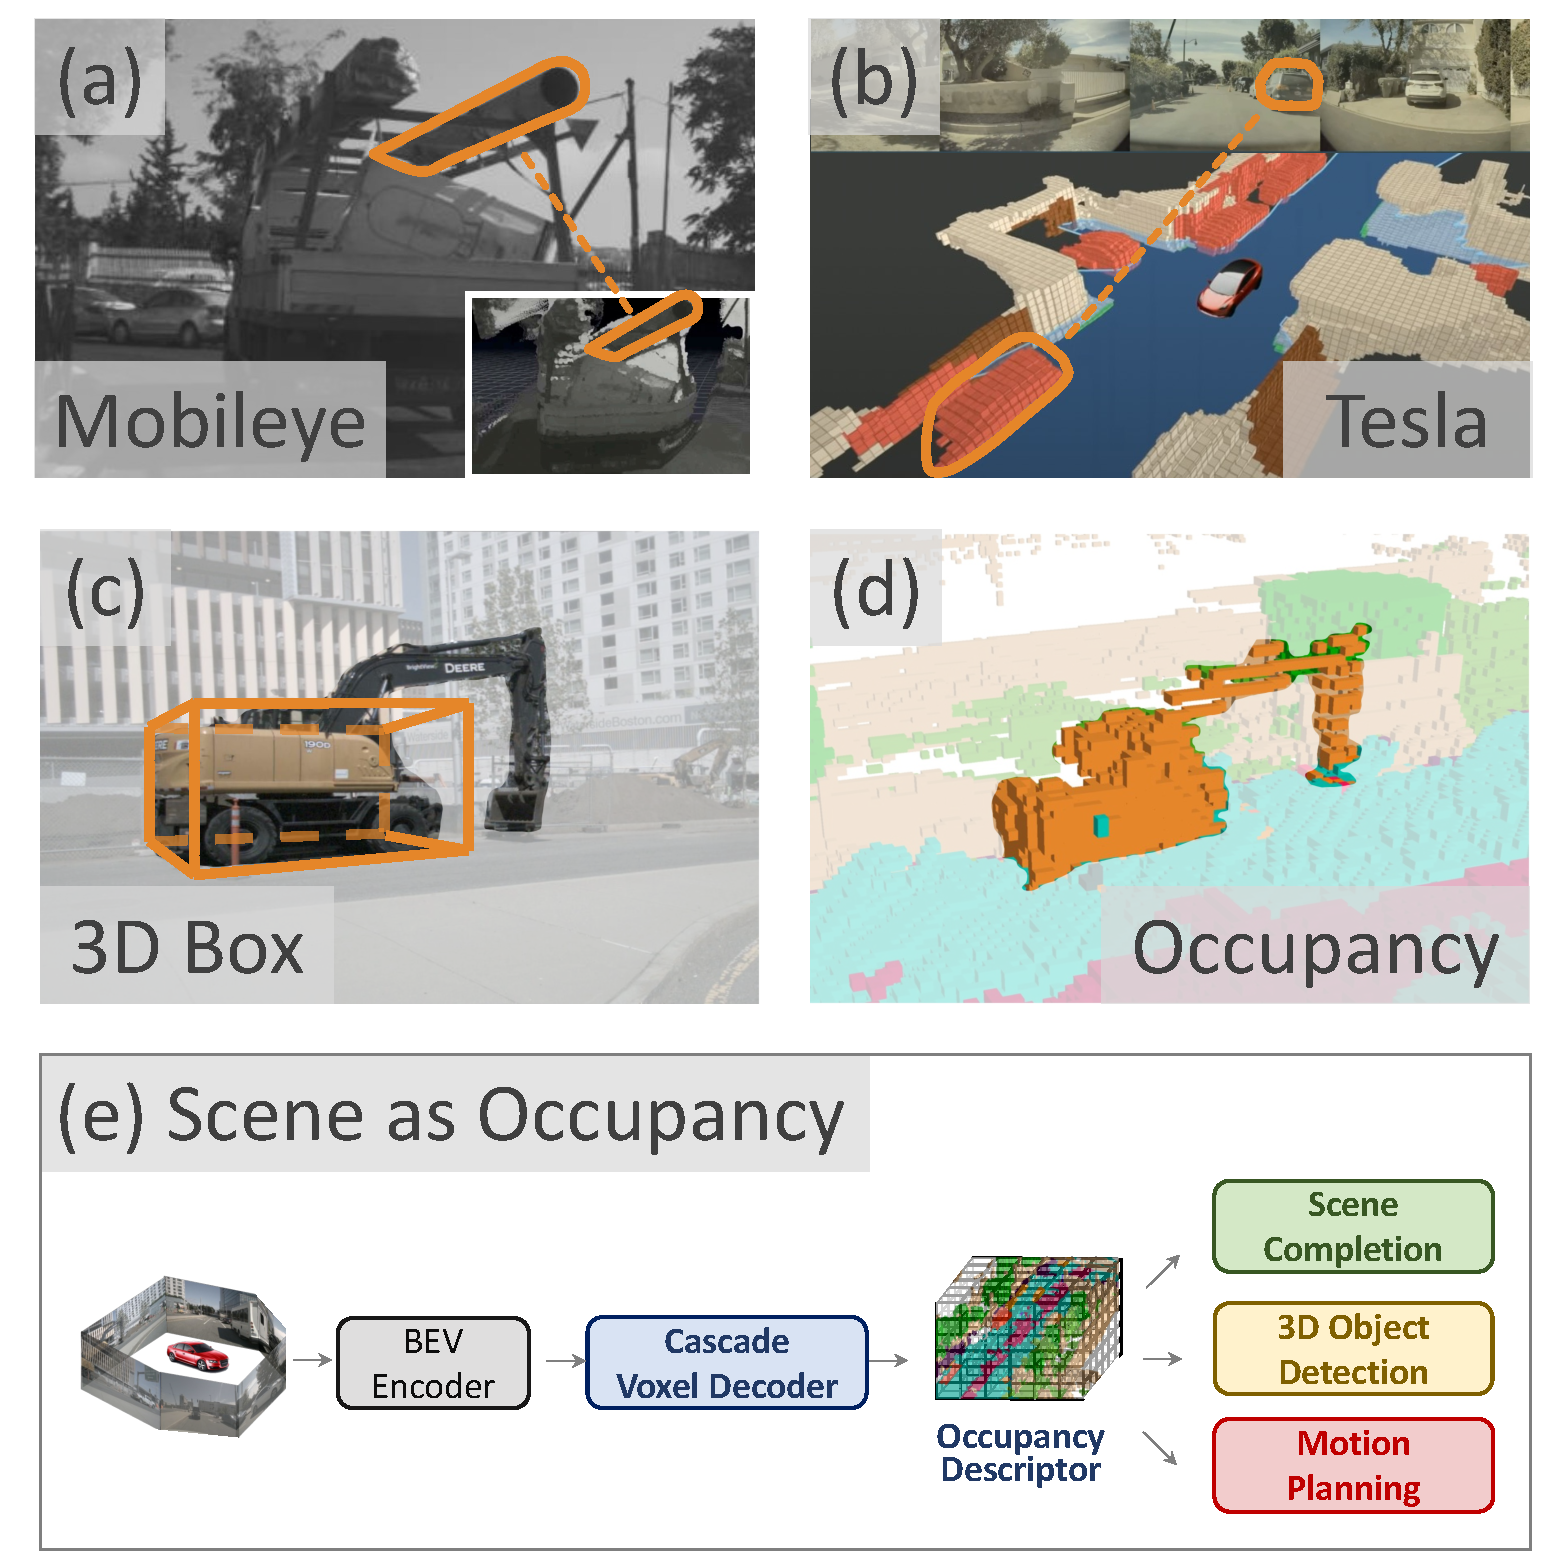
\includegraphics[width=0.72\linewidth]{ch-occnet/images/fig_motivation_v7_used.pdf}
  \caption[Scene as occupancy]{\textbf{Scene as occupancy.} Industry has endorsed representing objects with ViDAR~(a) or 3D occupancy~(b), because a conventional 3D bounding box cannot describe irregular vehicles in daily driving scenes in detail, \eg the protruding load in~(a) or the crane arm in~(c). Defining the 3D world as occupancy~(d) represents such obstacles better and helps avoid collisions. This chapter envisions occupancy as a general scene descriptor~(e) for a wide span of driving tasks beyond detection, such as planning.}
  \label{occnet:fig:motivation}
\end{figure}

For a human driver, describing the surrounding scene in 3D comes almost for free. A driver would say ``there is a Benz on the left side of my car, in around 5 inches'', or ``there is a truck carrying a huge protruding gas pipe on the rear, around 50 metres ahead''. Being able to describe the real world in such a ``there is'' form is essential for safe autonomous driving. It is non-trivial for a vision-centric system because of the diversity of entities in a street scene: vehicles such as cars, SUVs and construction trucks, static barriers, pedestrians, and background buildings and vegetation.

Quantising the 3D scene into structured cells with semantic labels attached, which we term 3D occupancy, is an intuitive way to produce such a description, and industry has advocated this form: Mobileye~\cite{mobile2020ces} and Tesla~\cite{tesla_ai_day} represent the scene with ViDAR and with occupancy, respectively (Fig.~\ref{occnet:fig:motivation}(a)--(b)). Compared with a 3D box, which oversimplifies the shape of an object, occupancy is geometry-aware: it depicts objects and background of different shapes as collections of cubes with different geometric structures. As Fig.~\ref{occnet:fig:motivation}(c)--(d) illustrates, a 3D box can describe only the main body of a construction vehicle, whereas occupancy preserves the detail of its crane arm.

\begin{table}[t]
  \centering
  \caption[Comparison of scene representations]{\textbf{Comparison of scene representations.} 3D occupancy unifies foreground objects and background stuff in a fine-grained, dense voxel space, and it is agnostic to the input modality.}
  \label{occnet:tab:compare_to_other_form}
  \small
  \begin{tabular}{lccccc}
    \toprule
    Representation & \makecell{Output\\space} & \makecell{Foreground\\object} & \makecell{Background\\\& mapping} & \makecell{Description\\granularity} & \makecell{Requires point\\cloud input} \\
    \midrule
    3D box      & 3D  & \checkmark & --         & 0.4--12\,m     & --         \\
    BEV seg.    & BEV & \checkmark & \checkmark & 0.5--1\,m      & --         \\
    Point cloud & 3D  & \checkmark & --         & $\sim$0.02\,m  & \checkmark \\
    \midrule
    \rowcolor{perceive!10} 3D occupancy & 3D & \checkmark & \checkmark & 0.25--0.5\,m & -- \\
    \bottomrule
  \end{tabular}
\end{table}

Table~\ref{occnet:tab:compare_to_other_form} compares occupancy with the representations that are widely deployed in driving. A 3D box covers only foreground objects. Point-cloud segmentation offers the finest granularity, around 0.02\,m, but requires LiDAR input and is therefore limited by cost. BEV segmentation covers objects and background, but its lack of a height dimension limits its granularity. Occupancy unifies foreground objects and background stuff in a dense 3D voxel space with a granularity of 0.25--0.5\,m, without requiring a point cloud as input. These advantages call for an investigation of whether occupancy can improve conventional perception tasks and downstream planning.

Occupancy has been discussed before, but only at an initial stage. In robotics, the occupancy grid map is a typical representation for mobile navigation~\cite{moras2015grid}, but it serves only as the search space of planning. In computer vision, 3D semantic scene completion (SSC)~\cite{song2016ssc} can be regarded as a perception task that evaluates the idea of occupancy. Vision-based methods for this task~\cite{huang2023tri,li2023voxformer,cao2022monoscene,miao2023occdepth} leave two opportunities open. They do not exploit temporal information, although history frames are an intuitive geometric prior for a vision-centric model that has to reconstruct geometry-aware occupancy. And, being one-stage methods~\cite{huang2023tri,miao2023occdepth,cao2022monoscene}, they ignore a coarse-to-fine scheme, which can improve the 3D geometric representation at an affordable cost. Beyond model design, the community still lacks a practical way to evaluate occupancy in a full-stack spirit, as vision-centric pipelines that connect perception to planning~\cite{hu2023uniad} prevail.

To address these issues, we propose OccNet, a multi-view, vision-centric pipeline with a cascade voxel decoder that reconstructs 3D occupancy with the aid of temporal clues, followed by task-specific heads for a wide range of driving tasks. The core of OccNet is a compact and representative occupancy embedding of the 3D scene. Rather than generating voxel features directly from image features, or using BEV features alone as in previous work~\cite{li2022bevformer,chen2022persformer,wang2022monocular}, OccNet decodes the occupancy feature from the BEV feature in a cascade fashion. The decoder recovers the height information progressively with voxel-based temporal self-attention and spatial cross-attention, bundled with a 3D deformable attention module for efficiency. Equipped with this descriptor, OccNet supports 3D occupancy prediction, 3D detection and BEV segmentation, and it facilitates motion planning. For a fair comparison across methods, we build OpenOcc, a benchmark with dense and high-quality annotations on the nuScenes dataset~\cite{caesar2020nuscenes,fong2022panoptic}. It comprises 34,149 annotated frames with over 1.4 billion occupancy cells, each assigned one of 16 classes that describe foreground objects and background stuff. It also annotates the motion of objects with directional flow, which makes it extensible to planning.

Evaluating OccNet on OpenOcc, we find that occupancy is superior to conventional representations in three respects.
\begin{itemize}
  \item \emph{Better perception.} Occupancy helps vision-only models acquire 3D geometry. A camera-only OccNet segments point clouds with an accuracy comparable to a LiDAR-based method, and pre-training or joint training with occupancy improves 3D detection. On semantic scene completion, OccNet improves the mIoU of TPVFormer~\cite{huang2023tri} by 14\% relative. Fine-tuned on small subsets of the training data, a detector pre-trained with OccNet outperforms one pre-trained with FCOS3D~\cite{wang2021fcos3d} by up to about 10 points.
  \item \emph{Better planning.} More accurate perception translates into better planning. Planning on predicted occupancy lowers the collision rate compared with planning on predicted 3D boxes or on BEV segmentation, by up to 58\%.
  \item \emph{Dense is better.} Dense occupancy supervises vision-only models more effectively than a sparse one.
\end{itemize}

%-----------------------------------------------------------------------
\section{Related Work}\label{occnet:sec:related}

This section positions occupancy against the output representations of driving perception and against the tasks closest to it. Broader background on camera-based 3D perception is given in Chapter~\ref{ch:background} and in the survey of BEV perception~\cite{li2023bevdevils}.

\paragraph{3D object detection.} Most detectors~\cite{Shi2020PVRCNNPF,wang2021fcos3d,li2022bevformer,liu2022bevfusion} adopt 3D boxes as the output of perception, since the box form is well structured for downstream rule-based approaches. Such a representation abstracts objects of different shapes into standardised cuboids; it therefore cares only about foreground objects and oversimplifies their shapes. Occupancy, in contrast, is a fine-grained description of the physical world that can differentiate objects of various shapes.

\paragraph{LiDAR segmentation.} LiDAR segmentation~\cite{zhu2021cylindrical,milioto2019rangenet++} addresses point-level 3D scene understanding. It requires a point cloud as input, which is expensive and less portable. Since LiDAR inherently suffers from a limited sensing range and a sparse coverage of the scene, such a pipeline is not well suited to holistic semantic understanding of the 3D scene~\cite{song2016ssc}.

\paragraph{BEV segmentation.} BEV segmentation~\cite{zhou2022cross,li2021hdmapnet} implicitly squeezes the height information into each cell of the BEV map. In challenging urban settings, however, explicit height information is necessary to capture entities above the ground, \eg traffic lights and overpasses. Occupancy, as an alternative, is aware of 3D geometry.

\paragraph{3D reconstruction and rendering.} Inferring the 3D geometry of objects or scenes from 2D images~\cite{Hartley2004,mildenhall2020nerf} has been a prevalent yet challenging problem in computer vision for many years. Most approaches in this domain~\cite{mueller2022instant,cao2022scenerf,Tancik2022blocknerf} cope with a single object or scene, which is not feasible for driving, where strong generalisation is required. Moreover, 3D reconstruction and rendering concentrate on the quality of the scene geometry and of the visual appearance, and pay less attention to model efficiency and semantic understanding.

\paragraph{Semantic scene completion.} The occupancy prediction studied in this chapter most resembles SSC~\cite{song2016ssc}. MonoScene~\cite{cao2022monoscene} first adopted a U-Net to infer dense 3D occupancy with semantic labels from a single monocular RGB image. Several related methods appeared concurrently with our work. VoxFormer~\cite{li2023voxformer} uses depth estimation to set voxel queries in a two-stage framework. OccDepth~\cite{miao2023occdepth} also follows a depth-aware design, in a stereo setting with distillation, to predict semantic occupancy. TPVFormer~\cite{huang2023tri} uses LiDAR-based sparse occupancy as supervision and proposes a tri-perspective view representation to obtain features. Wang \etal~\cite{wang2023openoccupancy} provide a carefully human-crafted occupancy benchmark for the community. Many of these works were developed on SemanticKITTI~\cite{behley2019semantickitti} and NYUv2~\cite{Silberman2012nyuv2}, with monocular or RGB-D input, a setting different from ours. More importantly, prior and concurrent works unanimously neglect temporal context. Using history voxel features is straightforward and has been verified by Tesla~\cite{tesla_ai_day}, yet no technical details or reports have been made public. Moreover, we position this work as the first to investigate occupancy as a general descriptor that can improve multiple tasks beyond detection.

%-----------------------------------------------------------------------
\section{OccNet}\label{occnet:sec:method}

\begin{figure}[t]
  \centering
  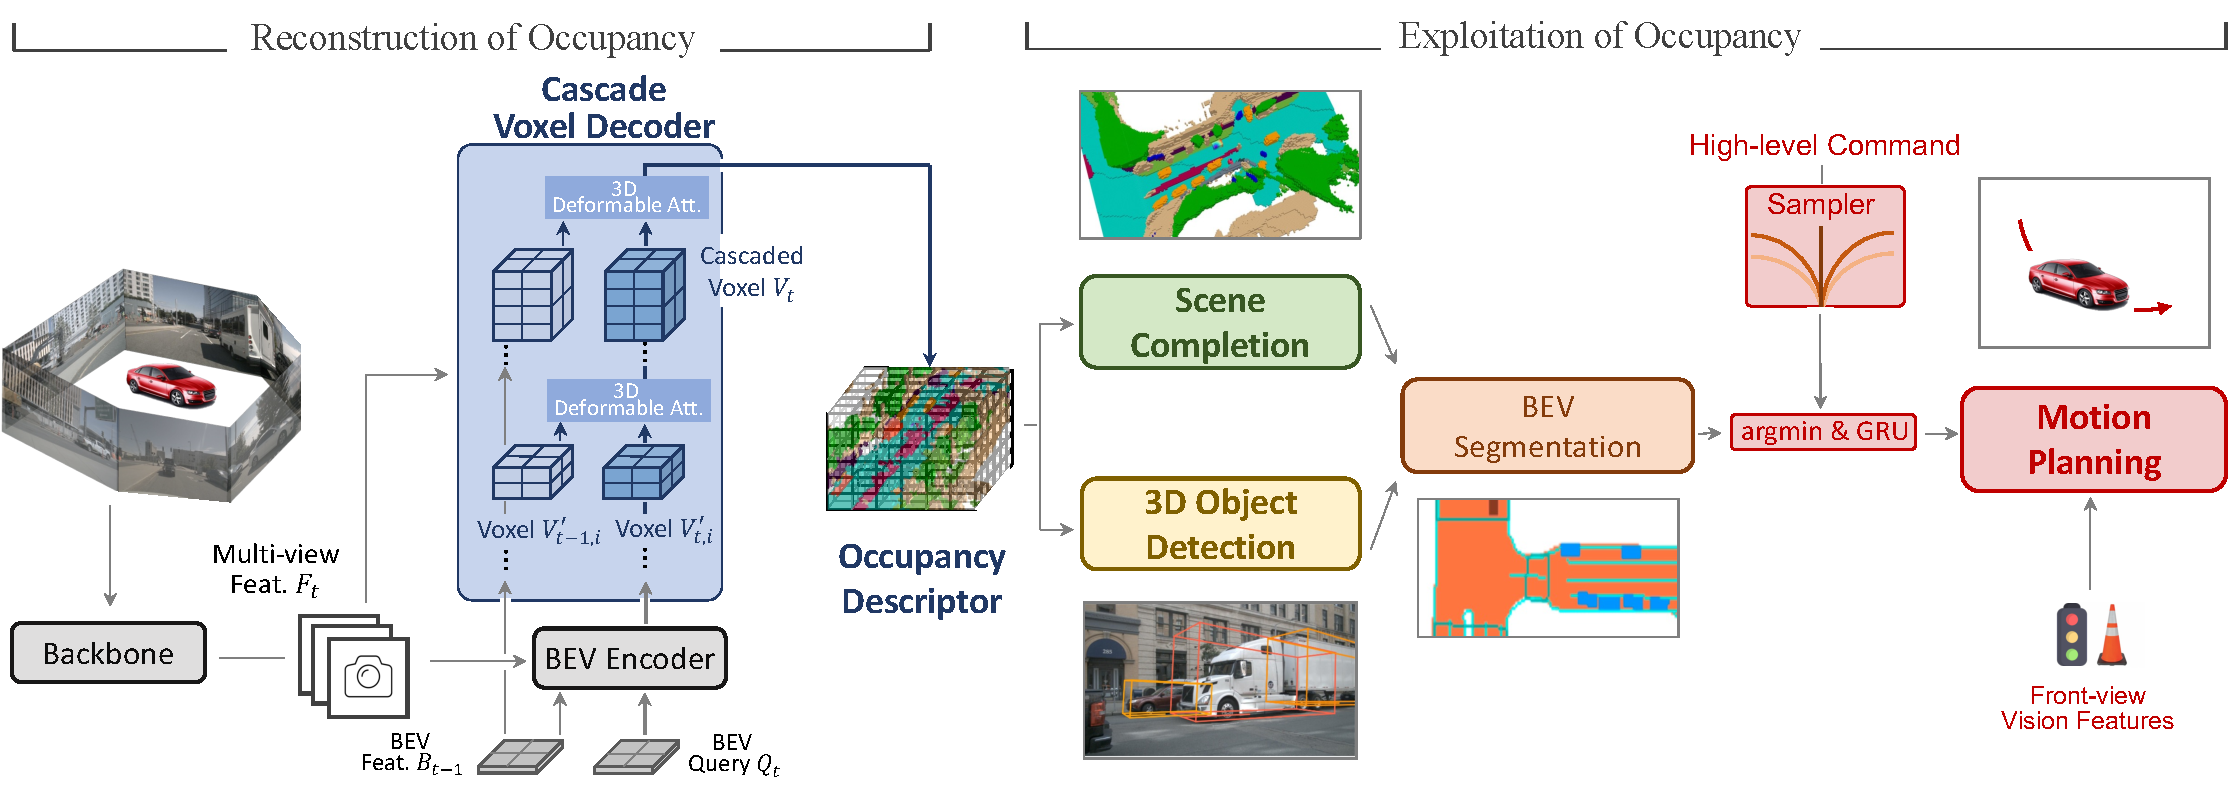
\includegraphics[width=\linewidth]{ch-occnet/images/fig_pipeline_overview_v8_used.pdf}
  \caption[The OccNet pipeline]{\textbf{The OccNet pipeline.} OccNet obtains a representative occupancy descriptor and applies it to various driving tasks, in two stages. \textbf{I.~Reconstruction of occupancy.} Given multi-view images, a BEV encoder first generates BEV features. The voxel decoder then operates in a cascade fashion, refining voxels progressively; a 3D deformable attention unit plays the role that deformable attention plays in 2D. Temporal voxels $V'_{t-1,i}$ are also incorporated. Some connections are omitted for brevity. \textbf{II.~Exploitation of occupancy.} The occupancy descriptor supports tasks such as semantic scene completion and 3D object detection. Compacting their outputs in BEV space yields a BEV segmentation map, which is fed directly into the planning pipeline~\cite{st-p32022}.}
  \label{occnet:fig:framework}
\end{figure}

OccNet obtains occupancy features from images and supports multiple driving tasks, as shown in Fig.~\ref{occnet:fig:framework}. It comprises two stages, the \emph{reconstruction of occupancy} and the \emph{exploitation of occupancy}. We term the part that bridges them the \emph{occupancy descriptor}, a unified description of the driving scene.

\paragraph{Reconstruction of occupancy.} The goal of this stage is a representative occupancy descriptor that supports downstream tasks. Motivated by the fast development of BEV perception~\cite{li2022bevformer,chen2022persformer,liang2022bevfusion}, OccNet is designed to carry this progress over to voxel-wise prediction in 3D space. Two extreme designs are possible. Using the BEV feature alone in downstream tasks is the simplest architecture, but it is not suitable for height-aware tasks in 3D space. At the other extreme, constructing voxel features directly from images incurs a huge computational cost. We term these two extremes \emph{BEVNet} and \emph{VoxelNet}; OccNet strikes a balance between them, achieving the best performance at an affordable cost (Section~\ref{occnet:sec:analysis}). The reconstruction stage first extracts multi-view features $F_t$ from the surround-view images and feeds them, together with the history BEV feature $B_{t-1}$ and the current BEV query $Q_t$, into a BEV encoder. The encoder follows the structure of BEVFormer~\cite{li2022bevformer}: $B_{t-1}$, $Q_t$ and $F_t$ pass through a spatial-temporal transformer block that produces the current BEV feature $B_t$. The image feature and the history and current BEV features are then decoded together into the occupancy descriptor by the \emph{cascade voxel decoder} of Section~\ref{occnet:sec:cascade_voxel_decoder}.

\paragraph{Exploitation of occupancy.} A wide range of driving tasks can be built on the reconstructed occupancy descriptor. Inspired by UniAD~\cite{hu2023uniad}, we prefer an explicit design for each representation. 3D semantic scene completion~\cite{song2016ssc} and 3D object detection are attached directly to the occupancy descriptor. Squeezing the 3D occupancy grid and the 3D boxes along the height axis yields a BEV segmentation map. This map is fed into the motion planning head together with a sampler conditioned on the high-level command, and the ego trajectory results from an \emph{argmin} over the sampled trajectories followed by a GRU module. Section~\ref{occnet:sec:exploitation_of_occupancy} details the task heads.

\subsection{Cascade Voxel Decoder}\label{occnet:sec:cascade_voxel_decoder}

To obtain a better voxel feature effectively and efficiently, we design a cascade structure in the decoder that recovers the height information of the voxel feature progressively.

\paragraph{From BEV to cascaded voxels.} Using the BEV feature directly, or reconstructing the voxel feature directly from the perspective view, costs performance or efficiency, respectively (see the ablation in Table~\ref{occnet:tab:efficiency}). We therefore break the reconstruction from the BEV feature $B_t\in\mathbb{R}^{H\times W\times C_{\text{BEV}}}$ to the desired voxel feature $V_t\in\mathbb{R}^{Z\times H\times W\times C_{\text{Voxel}}}$ into $N$ steps, which we call a cascade structure. Here $H$ and $W$ are the spatial dimensions of the BEV plane, $C_{\text{BEV}}$ and $C_{\text{Voxel}}$ are feature dimensions, and $Z$ is the desired height of the voxel space. We denote the intermediate voxel feature of the $i$-th step by $V'_{t,i}\in\mathbb{R}^{Z_i\times H\times W\times C_i}$. Along the cascade, the height $Z_i$ grows towards $Z$ while the channel number $C_i$ shrinks from $C_{\text{BEV}}$ towards $C_{\text{Voxel}}$; the schedule used in our experiments is given in Section~\ref{occnet:sec:exp_setup}. As shown in Fig.~\ref{occnet:fig:framework}, $B_{t-1}$ and $B_t$ are lifted to $V'_{t-1,i}$ and $V'_{t,i}$ by a feed-forward network and pass through the $i$-th voxel decoder, which outputs a refined $V'_{t,i}$; the later steps follow the same scheme, with an MLP transforming the feature dimension from $Z_i\times C_i$ to $Z_{i+1}\times C_{i+1}$ between consecutive steps (Appendix~\ref{occnet:app:implementation}). Each voxel decoder comprises a voxel-based temporal self-attention module, which refines $V'_{t,i}$ with the history feature $V'_{t-1,i}$, and a voxel-based spatial cross-attention module, which refines it with the image feature $F_t$. Step by step, the model increases $Z_i$ and decreases $C_i$, learning the final occupancy descriptor $V_t$ effectively and efficiently.

\paragraph{Voxel-based temporal self-attention.} Temporal information is crucial for representing the driving scene accurately~\cite{li2022bevformer}. Given the history voxel feature $V'_{t-1,i}$, we align it to the current occupancy feature $V'_{t,i}$ using the position of the ego vehicle. In standard self-attention, each query attends to every key and value, so the computational cost is huge, and in 3D space it grows by a factor of $Z^2$ compared with the 2D case. To alleviate this burden, we design an efficient voxel-based attention, termed \emph{3D deformable attention} (3D-DA). Applied in the voxel-based temporal self-attention, it lets each voxel query interact only with local voxels of interest, which keeps the computational cost affordable.

\paragraph{3D deformable attention.} We extend 2D deformable attention~\cite{Zhu2021DeformableDD} to 3D. Given a voxel feature $V'_{t,i}\in\mathbb{R}^{Z_i\times H\times W\times C_i}$, a voxel query with feature $\boldsymbol{q}\in\mathbb{R}^{C_i}$ and a 3D reference point $\boldsymbol{p}$, 3D deformable attention is computed as
\begin{equation}
  \operatorname{3D-DA}(\boldsymbol{q},\boldsymbol{p},V'_{t,i})
  = \sum_{m=1}^{M} W_m \sum_{k=1}^{K} A_{mk}\, W'_k\, V'_{t,i}(\boldsymbol{p}+\Delta\boldsymbol{p}_{mk}),
  \label{occnet:eq:3dda}
\end{equation}
where $M$ is the number of attention heads, $K\ll Z_iHW$ is the number of sampled keys, $W_m\in\mathbb{R}^{C_i\times(C_i/M)}$ and $W'_k\in\mathbb{R}^{(C_i/M)\times C_i}$ are learnable weights, $A_{mk}$ is the normalised attention weight, and $\boldsymbol{p}+\Delta\boldsymbol{p}_{mk}$ is the learnable sampling location in 3D space, at which the feature is computed from the voxel feature by trilinear interpolation.

\paragraph{Voxel-based spatial cross-attention.} In the cross-attention, the voxel feature $V'_{t,i}$ interacts with the multi-scale image features $F_t$ through 2D deformable attention~\cite{Zhu2021DeformableDD}. The $i$-th decoder samples $N_{\text{ref},i}$ 3D points directly from each voxel, projects them to the image views, and interacts with the sampled image features. Whereas a BEV query in BEVFormer~\cite{li2022bevformer} samples its reference points along a pillar, this design maintains the height information and ensures that a voxel-wise feature is learned.

\subsection{Exploiting Occupancy for Driving Tasks}\label{occnet:sec:exploitation_of_occupancy}

OccNet depicts the scene in 3D space with a fine-grained occupancy descriptor, which can be fed into various driving tasks without excessive computational overhead.

\paragraph{Semantic scene completion.} For simplicity, an MLP head predicts the semantic label of each voxel. It is trained with the focal loss~\cite{Lin2017FocalLF} to balance the huge numerical imbalance between occupied and empty voxels. In addition, a flow head trained with an $L_1$ loss estimates the flow velocity of each occupied voxel.

\paragraph{3D object detection.} Inspired by the head design of BEVFormer~\cite{li2022bevformer}, we compact the occupancy descriptor into BEV and apply a query-based detection head, a variant of Deformable DETR~\cite{Zhu2021DeformableDD}, to predict 3D boxes.

\paragraph{BEV segmentation.} Following the spatial-temporal fusion perception structure of ST-P3~\cite{st-p32022}, map representation and semantic segmentation are predicted from the BEV feature, as in 3D object detection. The BEV segmentation head comprises a drivable-area head and a lane head for the map representation, and a vehicle segmentation head and a pedestrian segmentation head for semantic segmentation.

\paragraph{Motion planning.} For planning, either the occupancy predicted by SSC or the predicted 3D boxes are transformed into a BEV segmentation map (Fig.~\ref{occnet:fig:framework}). The occupancy, or the set of boxes, is squeezed along the height dimension, and the semantic labels of each BEV cell are turned into a binary format, where 1 indicates that the cell is occupied and 0 that it is empty. This map enters the safety cost function, and the safety, comfort and progress costs are computed for the sampled trajectories. Compared with 3D boxes, the richer background information of occupancy leads to a more comprehensive safety cost, so the safety cost value has to be normalised between the two kinds of BEV maps. All candidate trajectories are sampled with random velocity, acceleration and curvature. Under the guidance of a high-level command (forward, turn left or turn right), the trajectory with the lowest cost for that command is selected. A GRU refinement that uses the front-view vision feature, as in ST-P3~\cite{st-p32022}, then produces the final trajectory.

%-----------------------------------------------------------------------
\section{The OpenOcc Benchmark}\label{occnet:sec:benchmark}

To evaluate occupancy fairly across methods, we introduce OpenOcc, which at the time of publication was the first dense, high-quality 3D occupancy benchmark built on top of the widely used nuScenes dataset~\cite{caesar2020nuscenes,fong2022panoptic}. Compared with existing counterparts such as SemanticKITTI~\cite{behley2019semantickitti}, which provides only a front camera, OpenOcc provides surround-view camera images with the corresponding 3D occupancy and flow annotations.

\subsection{Benchmark Overview}\label{occnet:sec:benchmark_overview}

OpenOcc provides dense, high-quality occupancy annotations generated from the sparse LiDAR data and the 3D boxes of nuScenes. It comprises 34,149 annotated frames covering all 700 training and 150 validation scenes. Over 1.4 billion voxels are annotated with 16 classes: 10 foreground object classes (barrier, bicycle, bus, car, construction vehicle, motorcycle, pedestrian, traffic cone, trailer and truck) and 6 background stuff classes (driveable surface, other flat, sidewalk, terrain, manmade and vegetation). In addition, the motion of foreground objects is captured by flow annotations on the object voxels. Occupancy is defined within the volume $\mathcal{V}=[-50\,\text{m},50\,\text{m}]\times[-50\,\text{m},50\,\text{m}]\times[-5\,\text{m},3\,\text{m}]$ in the LiDAR coordinate system, voxelised at a resolution of $\Delta s=0.5$\,m into $200\times200\times16$ voxels.

\begin{table}[t]
  \centering
  \caption[Comparison of OpenOcc with existing occupancy benchmarks]{\textbf{Comparison of OpenOcc with existing benchmarks.} \emph{Multi-view}: the dataset uses multi-view images as input. \emph{Flow}: flow annotations are provided. \emph{Density}: voxel density of the annotations.}
  \label{occnet:tab:compare_gt}
  \begin{tabular}{lcccc}
    \toprule
    Dataset & Multi-view & Scenes & Flow & Density \\
    \midrule
    SemanticKITTI~\cite{behley2019semantickitti} & --         & 22  & -- & --           \\
    SparseOcc~\cite{huang2023tri}                & \checkmark & 850 & -- & $\sim$0.11   \\
    OccData~\cite{Fang2023}                      & \checkmark & 850 & -- & $\sim$0.76   \\
    \midrule
    \rowcolor{perceive!10} OpenOcc (ours)        & \checkmark & 850 & \checkmark & 1    \\
    \bottomrule
  \end{tabular}
\end{table}

\begin{figure}[t]
  \centering
  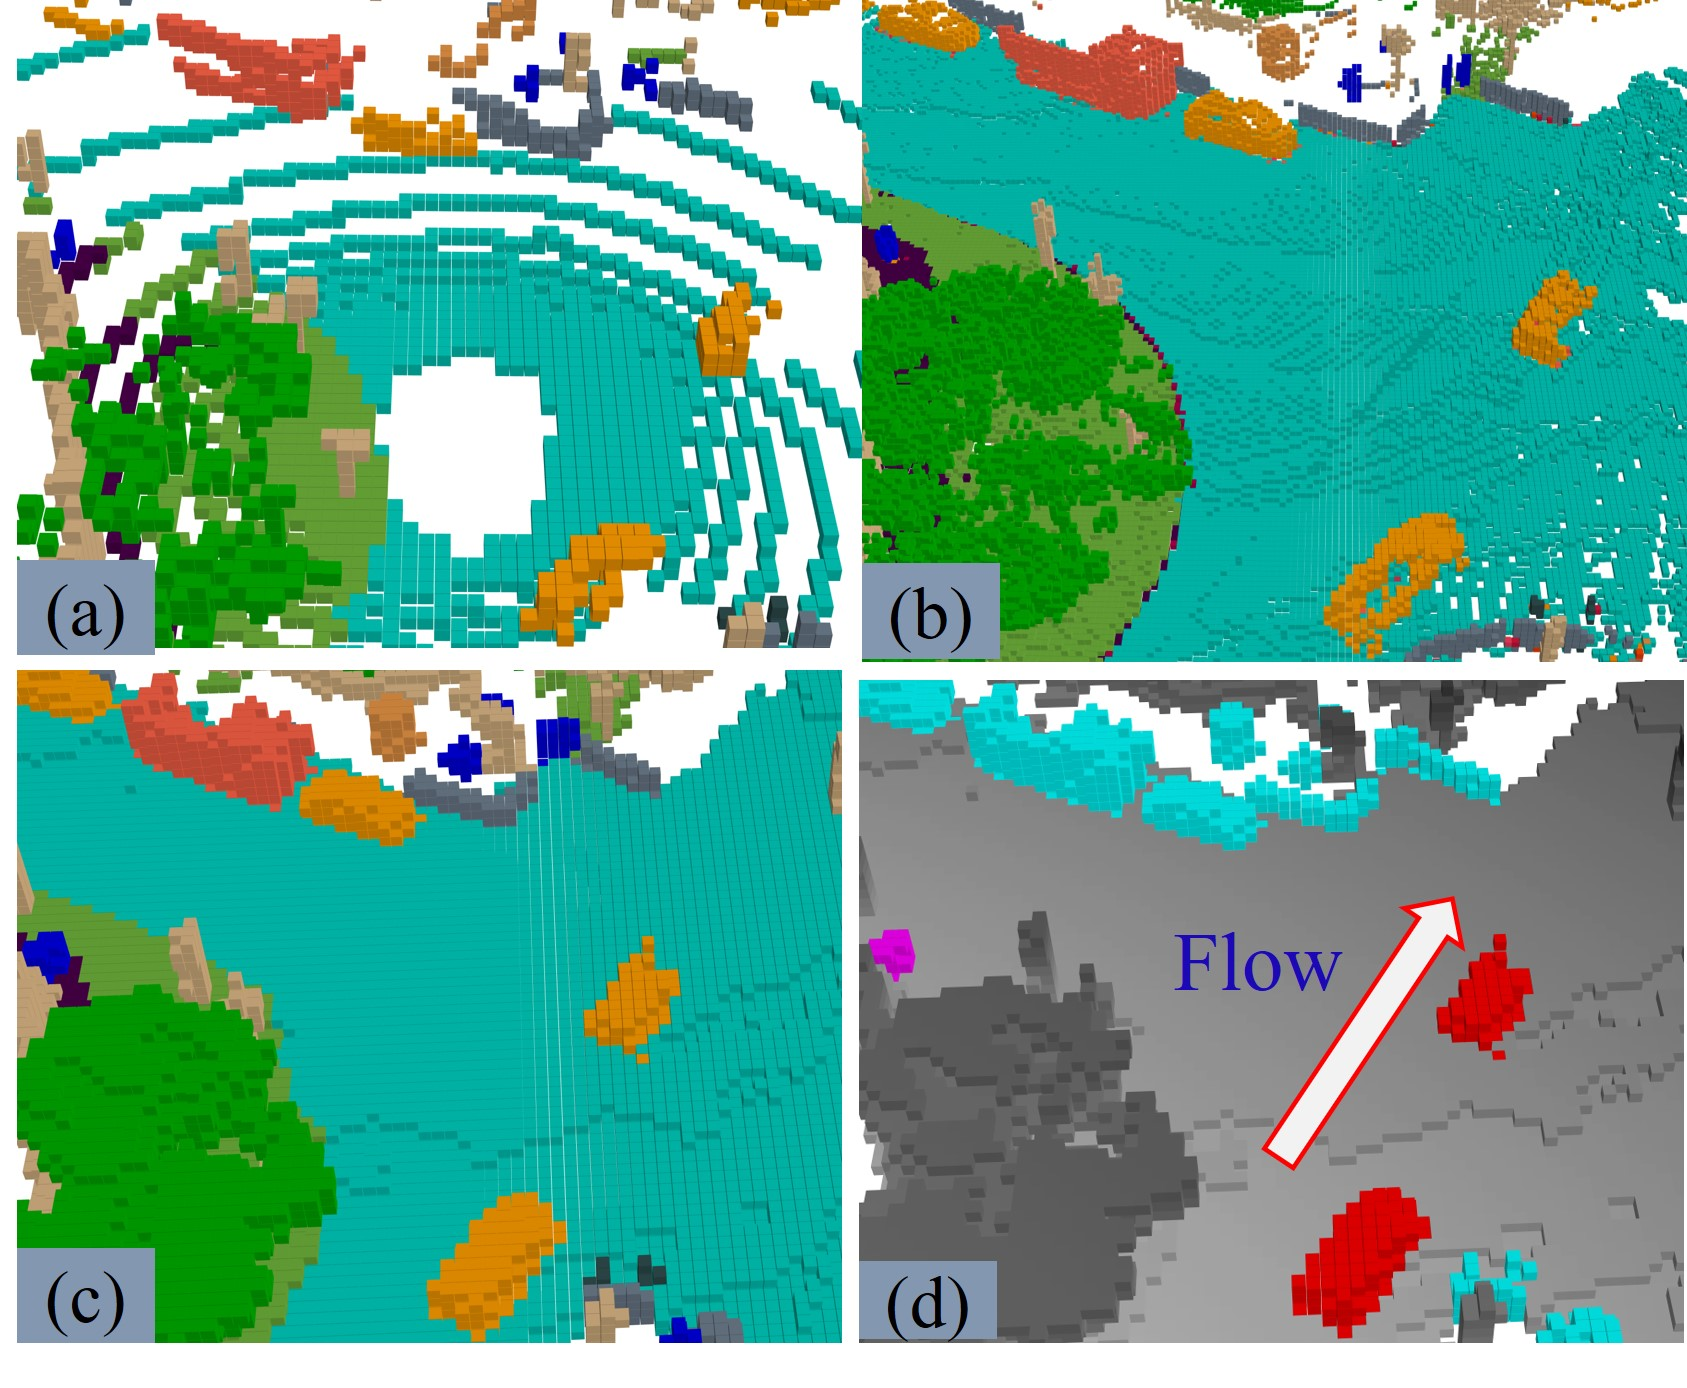
\includegraphics[width=0.68\linewidth]{ch-occnet/images/fig_compare_dataset_used.jpg}
  \caption[Visual comparison of 3D occupancy annotations]{\textbf{Visual comparison of 3D occupancy annotations.} Compared with (a)~sparse occupancy~\cite{huang2023tri} and (b)~OccData~\cite{Fang2023}, OpenOcc provides (c)~dense and high-quality annotations with (d)~additional flow annotations for foreground objects, which can be used for motion planning.}
  \label{occnet:fig:compare_gt}
\end{figure}

Table~\ref{occnet:tab:compare_gt} compares OpenOcc with other benchmarks: it provides the most complete description of the scene, including occupancy and flow. As Fig.~\ref{occnet:fig:compare_gt} shows, SparseOcc~\cite{huang2023tri} voxelises only the sparse LiDAR data of the key frames, which is too sparse to represent the 3D scene. OpenOcc, in contrast, represents the complete scene with flow information and captures fine-grained local geometry with high quality. Statistics of the class distribution and of object motion are given in Appendix~\ref{occnet:app:openocc}.

\subsection{Generating High-Quality Annotations}\label{occnet:sec:annotation}

\paragraph{Independent accumulation of background and foreground.} To generate a dense representation, it is intuitive to accumulate all the sparse LiDAR points of the key frames and intermediate frames~\cite{behley2019semantickitti}. Directly accumulating points from intermediate frames by coordinate transformation is problematic, however, because of moving objects. We therefore split the LiDAR points into static background points and foreground points using the 3D boxes, and accumulate the two separately: the static background points in the global world coordinate system, and the object points in the coordinate system of each object. Since nuScenes provides no boxes for intermediate frames, we approximate them by linear interpolation between the two adjacent key frames (Appendix~\ref{occnet:app:openocc}).

\paragraph{Generation of annotations.} Given the dense background and object points, we voxelise the 3D space and label each voxel by a majority vote of the labelled points inside it. Unlike existing benchmarks that provide only occupancy labels, we also annotate the flow velocity of each voxel from the velocity of its 3D box, to facilitate downstream tasks such as motion planning. Using key frames alone would leave the generated occupancy sparse, so we further annotate voxels that contain unlabelled LiDAR points from intermediate frames, based on the surrounding labelled voxels, which increases the density. Because nuScenes has the issue of missing translation along the $z$-axis, we refine the occupancy by completing the scene, \eg by filling holes in the road, for higher quality. Finally, we mark part of the voxels as invisible from the camera views by ray tracing, which makes the benchmark more suitable for camera-based tasks. Fig.~\ref{occnet:fig:occ_gt_pipeline} in Appendix~\ref{occnet:app:openocc} illustrates these steps.

%-----------------------------------------------------------------------
\section{Experiments}\label{occnet:sec:experiments}

\subsection{Experimental Setup}\label{occnet:sec:exp_setup}

\paragraph{Implementation.} Following the experimental setting of BEVFormer~\cite{li2022bevformer}, we use two backbones: ResNet50~\cite{he2016resnet} initialised from ImageNet~\cite{deng2009imagenet}, and ResNet101-DCN~\cite{he2016resnet} initialised from FCOS3D~\cite{wang2021fcos3d}. The BEV feature $B_t$ has $H=W=200$ and $C_{\text{BEV}}=256$. The decoder has $N=4$ occupancy feature maps $V'_{t,i}\in\mathbb{R}^{Z_i\times H\times W\times C_i}$ with $Z_i=2^i$, $C_1=C_2=128$ and $C_3=C_4=64$. The voxel-based spatial cross-attention samples $N_{\text{ref},i}=4$ points in each queried voxel. By default, OccNet is trained for 24 epochs with a learning rate of $2\times10^{-4}$, and the temporal self-attention uses two history frames. Further implementation details, including those of BEVNet and VoxelNet, are given in Appendix~\ref{occnet:app:implementation}.

\paragraph{Tasks and metrics.} Semantic scene completion is evaluated on OpenOcc with the mean intersection-over-union (mIoU) over the 16 classes and the class-agnostic geometric $\text{IoU}_{\text{geo}}$. LiDAR segmentation and 3D detection are evaluated on the nuScenes validation set, the latter with the official nuScenes detection metrics. BEV segmentation is evaluated by IoU, and planning follows ST-P3~\cite{st-p32022} in reporting the L2 distance to the ground-truth trajectory and the collision rate. Appendix~\ref{occnet:app:metrics} defines the metrics.

\subsection{Main Results}\label{occnet:sec:main_results}

\begin{table}[t]
  \centering
  \caption[Semantic scene completion on OpenOcc]{\textbf{3D occupancy prediction in terms of semantic scene completion.} Semantic (mIoU) and geometric ($\text{IoU}_{\text{geo}}$) metrics of camera-based models on OpenOcc. OccNet outperforms previous state-of-the-art methods in both. $^{\ast}$: trained and evaluated on OpenOcc.}
  \label{occnet:tab:occ_method}
  \setlength{\tabcolsep}{3.5pt}
  \resizebox{\textwidth}{!}{%
  \begin{tabular}{@{}llcc*{16}{c}@{}}
    \toprule
    Method & Backbone & $\text{IoU}_{\text{geo}}$ & mIoU & \rotatebox{90}{barrier} & \rotatebox{90}{bicycle} & \rotatebox{90}{bus} & \rotatebox{90}{car} & \rotatebox{90}{const.\ veh.} & \rotatebox{90}{motorcycle} & \rotatebox{90}{pedestrian} & \rotatebox{90}{traffic cone} & \rotatebox{90}{trailer} & \rotatebox{90}{truck} & \rotatebox{90}{driv.\ surf.} & \rotatebox{90}{other flat} & \rotatebox{90}{sidewalk} & \rotatebox{90}{terrain} & \rotatebox{90}{manmade} & \rotatebox{90}{vegetation} \\
    \midrule
    BEVDet4D~\cite{huang2022bevdet4d} & ResNet50 & 18.27 & 9.85 & 13.56 & 0.00 & 13.04 & 26.98 & 0.61 & 1.20 & 6.76 & 0.93 & 1.93 & 12.63 & 27.23 & 11.09 & 13.64 & 12.04 & 6.42 & 9.56 \\
    BEVDepth~\cite{li2022bevdepth} & ResNet50 & 23.45 & 11.88 & 15.15 & 0.02 & 20.75 & 27.05 & 1.10 & 2.01 & 9.69 & 1.45 & 1.91 & 14.31 & 31.92 & 7.88 & 17.08 & 16.27 & 8.76 & 14.75 \\
    BEVDet~\cite{huang2021bevdet} & ResNet50 & 27.46 & 12.49 & 16.06 & 0.11 & 18.27 & 21.09 & 2.62 & 1.42 & 7.78 & 1.08 & 3.4 & 13.76 & 33.89 & 10.84 & 17.55 & 22.03 & 11.72 & 18.15 \\
    \rowcolor{perceive!10} OccNet (ours) & ResNet50 & \textbf{37.69} & \textbf{19.48} & \textbf{20.63} & \textbf{5.52} & \textbf{24.16} & \textbf{27.72} & \textbf{9.79} & \textbf{7.73} & \textbf{13.38} & \textbf{7.18} & \textbf{10.68} & \textbf{18.00} & \textbf{46.13} & \textbf{20.6} & \textbf{26.75} & \textbf{29.37} & \textbf{16.90} & \textbf{27.21} \\
    \midrule
    TPVFormer$^{\ast}$~\cite{huang2023tri} & ResNet101 & 37.47 & 23.67 & 27.95 & 12.75 & 33.24 & \textbf{38.70} & 12.41 & 17.84 & 11.65 & 8.49 & \textbf{16.42} & \textbf{26.47} & 47.88 & 25.43 & 30.62 & 30.18 & 15.51 & 23.12 \\
    \rowcolor{perceive!10} OccNet (ours) & ResNet101 & \textbf{41.08} & \textbf{26.98} & \textbf{29.77} & \textbf{16.89} & \textbf{34.16} & 37.35 & \textbf{15.58} & \textbf{21.92} & \textbf{21.29} & \textbf{16.75} & 16.37 & 26.23 & \textbf{50.74} & \textbf{27.93} & \textbf{31.98} & \textbf{33.24} & \textbf{20.80} & \textbf{30.68} \\
    \bottomrule
  \end{tabular}}
\end{table}

\begin{figure}[t]
  \centering
  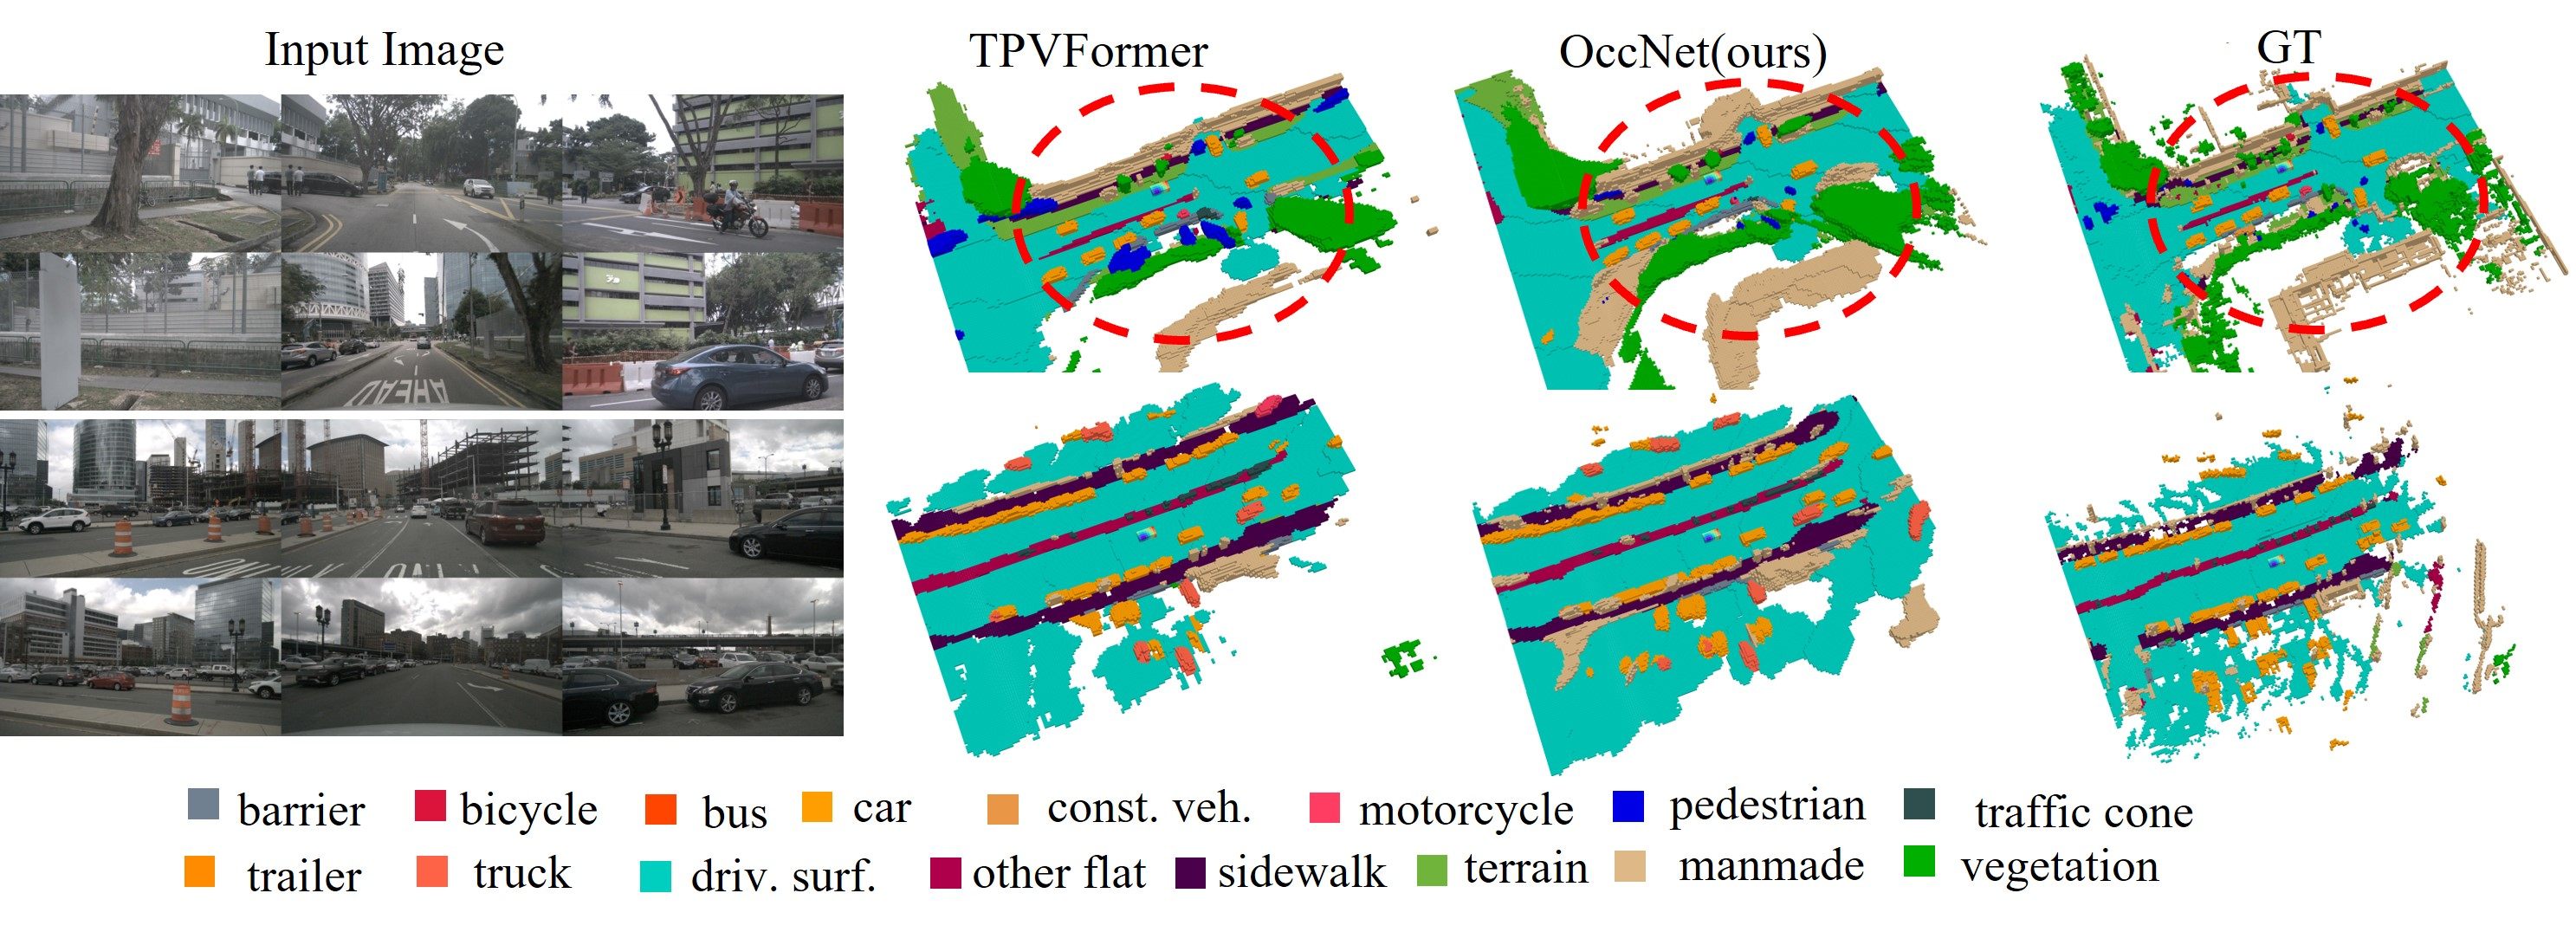
\includegraphics[width=\linewidth]{ch-occnet/images/fig_occ_gt_pred_used.jpg}
  \caption[Qualitative results of occupancy prediction]{\textbf{Qualitative results of occupancy prediction.} OccNet outperforms TPVFormer~\cite{huang2023tri} in scene detail and in the semantic classification of foreground objects, such as the pedestrian in the dashed region.}
  \label{occnet:fig:compare_occ_method}
\end{figure}

\paragraph{Semantic scene completion.} Table~\ref{occnet:tab:occ_method} and Fig.~\ref{occnet:fig:compare_occ_method} compare OccNet with previous state-of-the-art methods on semantic scene completion. We reproduce BEVDet4D~\cite{huang2022bevdet4d}, BEVDepth~\cite{li2022bevdepth} and BEVDet~\cite{huang2021bevdet} by replacing their detection heads with a scene completion head built on their BEV feature maps. OccNet outperforms these methods by a large margin: with ResNet50 it reaches 19.48 mIoU and 37.69 $\text{IoU}_{\text{geo}}$, whereas the best of them reaches 12.49 mIoU and 27.46 $\text{IoU}_{\text{geo}}$ (BEVDet). Compared with a BEV feature map, the occupancy descriptor is thus better suited to voxel-wise prediction. We also compare OccNet with TPVFormer~\cite{huang2023tri}, which was developed for surround-view 3D semantic occupancy prediction. OccNet surpasses it by 3.31 mIoU points (26.98 \vs 23.67), which indicates that the occupancy descriptor represents the scene better than TPV features. TPVFormer is better on car, truck and trailer, whose samples are relatively large in the benchmark, and for which its sampling strategy learns better features. For small objects such as pedestrians and traffic cones, however, OccNet outperforms TPVFormer by a large margin of about 10 points (21.29 \vs 11.65 and 16.75 \vs 8.49).

\begin{table}[t]
  \centering
  \caption[LiDAR segmentation on nuScenes from camera-only occupancy]{\textbf{LiDAR segmentation on the nuScenes validation set with OccNet (ResNet101).} With camera input, OccNet is comparable with a LiDAR-based method. $^{\ast}$: trained from scratch on OpenOcc.}
  \label{occnet:tab:lidarseg}
  \setlength{\tabcolsep}{3.5pt}
  \resizebox{\textwidth}{!}{%
  \begin{tabular}{@{}llc*{16}{c}@{}}
    \toprule
    Method & Input & mIoU & \rotatebox{90}{barrier} & \rotatebox{90}{bicycle} & \rotatebox{90}{bus} & \rotatebox{90}{car} & \rotatebox{90}{const.\ veh.} & \rotatebox{90}{motorcycle} & \rotatebox{90}{pedestrian} & \rotatebox{90}{traffic cone} & \rotatebox{90}{trailer} & \rotatebox{90}{truck} & \rotatebox{90}{driv.\ surf.} & \rotatebox{90}{other flat} & \rotatebox{90}{sidewalk} & \rotatebox{90}{terrain} & \rotatebox{90}{manmade} & \rotatebox{90}{vegetation} \\
    \midrule
    RangeNet++~\cite{milioto2019rangenet++} & LiDAR & 65.50 & 66.00 & 21.30 & 77.20 & 80.90 & 30.20 & 66.80 & 69.60 & 52.10 & 54.20 & 72.20 & 94.10 & 66.60 & 63.50 & 70.10 & 83.10 & 79.80 \\
    Cylinder3D~\cite{zhu2021cylindrical} & LiDAR & 76.10 & 76.40 & 40.30 & 91.20 & 93.80 & 51.30 & 78.00 & 78.90 & 64.90 & 62.10 & 84.40 & 96.80 & 71.60 & 76.40 & 75.40 & 90.50 & 87.40 \\
    \midrule
    TPVFormer$^{\ast}$~\cite{huang2023tri} & Camera & 58.45 & 65.99 & 24.50 & 80.88 & 74.28 & 47.04 & 47.09 & 33.42 & 14.52 & 53.96 & 70.79 & 88.55 & 61.63 & 59.46 & 63.15 & 75.76 & 74.17 \\
    \rowcolor{perceive!10} OccNet (ours) & Camera & 60.46 & 66.95 & 32.58 & 77.37 & 73.88 & 37.62 & 50.87 & 51.45 & 33.69 & 52.20 & 67.08 & 88.72 & 57.99 & 58.04 & 63.06 & 78.91 & 76.97 \\
    \bottomrule
  \end{tabular}}
\end{table}

\paragraph{Occupancy for LiDAR segmentation.} Occupancy is a voxelised representation of points in 3D space, and semantic scene completion becomes equivalent to semantic LiDAR segmentation as $\Delta s\to0$. We transfer the semantic occupancy prediction to LiDAR segmentation by assigning each point the label of its voxel, and evaluate the result with mIoU. As reported in Table~\ref{occnet:tab:lidarseg}, OccNet, given only camera input, is comparable with the LiDAR segmentation model RangeNet++~\cite{milioto2019rangenet++} in mIoU (60.46 \vs 65.50), and even outperforms it on bicycle (32.58 \vs 21.30). It also outperforms TPVFormer~\cite{huang2023tri} by 2 points in mIoU. A stronger LiDAR model, Cylinder3D~\cite{zhu2021cylindrical}, remains clearly ahead at 76.10 mIoU.

\begin{table}[t]
  \centering
  \caption[Joint training of 3D occupancy and 3D detection]{\textbf{Joint training of 3D occupancy and 3D detection} on the nuScenes validation set. Joint training with occupancy helps the detection task.}
  \label{occnet:tab:joint_train}
  \small
  \begin{tabular}{llccccccc}
    \toprule
    Model & Joint & mAP$\uparrow$ & NDS$\uparrow$ & mAOE$\downarrow$ & mAVE$\downarrow$ & mAAE$\downarrow$ & mATE$\downarrow$ & mASE$\downarrow$ \\
    \midrule
    \multirow{2}{*}{BEVNet}   & --         & 0.259 & 0.377 & 0.600 & 0.592 & 0.216 & \textbf{0.828} & \textbf{0.290} \\
                              & \checkmark & \textbf{0.271} & \textbf{0.390} & \textbf{0.578} & \textbf{0.541} & \textbf{0.211} & 0.835 & 0.293 \\
    \midrule
    \multirow{2}{*}{VoxelNet} & --         & 0.271 & 0.380 & 0.603 & 0.616 & 0.219 & 0.832 & \textbf{0.284} \\
                              & \checkmark & \textbf{0.277} & \textbf{0.387} & \textbf{0.586} & \textbf{0.614} & \textbf{0.203} & \textbf{0.828} & 0.285 \\
    \midrule
    \multirow{2}{*}{OccNet}   & --         & 0.276 & 0.382 & 0.655 & 0.588 & 0.209 & \textbf{0.817} & \textbf{0.290} \\
                              & \checkmark & \textbf{0.276} & \textbf{0.390} & \textbf{0.585} & \textbf{0.570} & \textbf{0.190} & 0.842 & 0.292 \\
    \bottomrule
  \end{tabular}
\end{table}

\paragraph{Occupancy for 3D detection.} In scene completion, the locations of foreground objects are coarsely regressed, which can help the box regression of 3D detection. Table~\ref{occnet:tab:joint_train} shows that jointly training scene completion and 3D detection improves NDS for all three of our models, BEVNet, VoxelNet and OccNet, and mAP for BEVNet and VoxelNet, while the mAP of OccNet is unchanged. The orientation, velocity and attribute errors decrease for all three models. The voxelised representation with $\Delta s=0.5$\,m, however, is too coarse for metrics that depend on the precise centre distance and IoU of 3D boxes, so joint training slightly increases the scale error of all three models and the translation error of BEVNet and OccNet.

\begin{figure}[t]
  \centering
  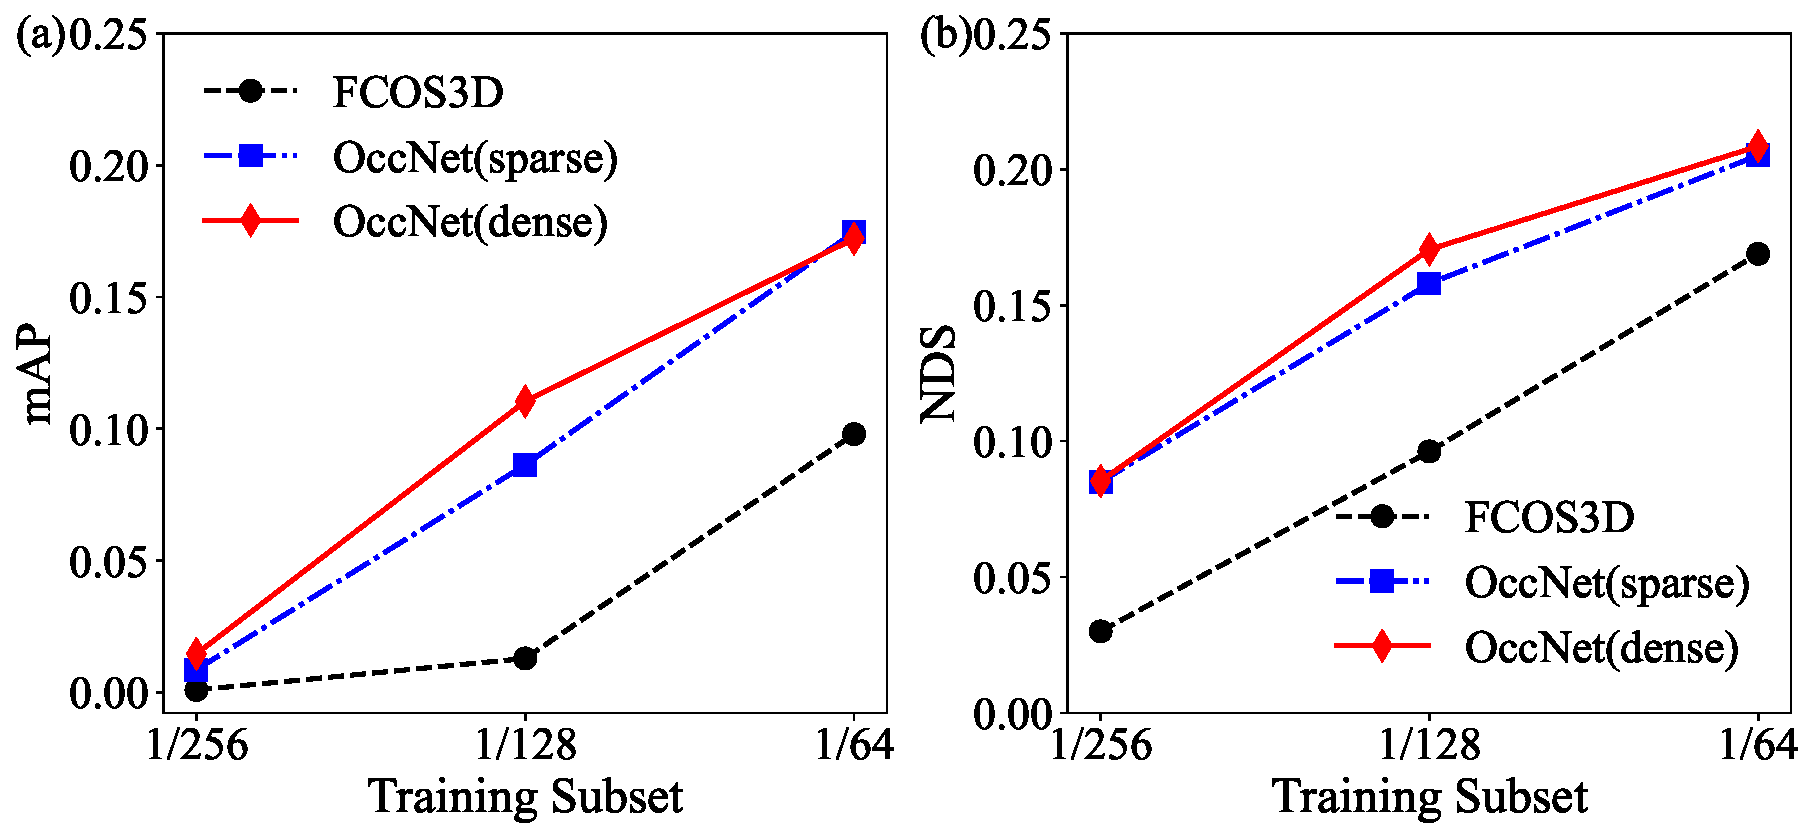
\includegraphics[width=0.9\linewidth]{ch-occnet/images/fig_compare_pretrain_v2_used.pdf}
  \caption[Detection performance with different pre-trained models and training-set sizes]{\textbf{Detection performance with different pre-trained models and training-set sizes.} (a)~mAP and (b)~NDS after fine-tuning on subsets of the training set. OccNet (sparse) and OccNet (dense) denote OccNet trained on sparse and dense occupancy data, respectively.}
  \label{occnet:fig:pretrain_for_detection}
\end{figure}

\begin{table}[t]
  \centering
  \caption[Pre-training tasks for BEV segmentation]{\textbf{Pre-training tasks for BEV segmentation} (IoU). Occupancy pre-training helps BEV segmentation achieve a higher IoU. The main value is the average of the four IoUs.}
  \label{occnet:tab:bev_seg}
  \begin{tabular}{lccccc}
    \toprule
    Pre-training & Main value & Drivable area & Lane & Vehicle & Pedestrian \\
    \midrule
    Det & 18.18 & 44.59 & 13.62 & 12.29 & 2.21 \\
    \rowcolor{perceive!10} Occ & \textbf{19.17} & \textbf{47.21} & \textbf{13.83} & \textbf{12.91} & \textbf{2.74} \\
    \bottomrule
  \end{tabular}
\end{table}

\paragraph{Pre-trained occupancy for 3D detection and BEV segmentation.} An OccNet trained on semantic scene completion obtains a general representation of 3D space, because the scene is reconstructed in its occupancy descriptor. The learned descriptor can therefore be transferred to downstream 3D perception tasks by fine-tuning. As Fig.~\ref{occnet:fig:pretrain_for_detection} shows, a detector pre-trained with OccNet outperforms one pre-trained with the FCOS3D~\cite{wang2021fcos3d} detector at every training-set scale considered (1/256, 1/128 and 1/64 of the training set), with gains of up to about 10 points. For BEV segmentation, occupancy pre-training also yields a higher IoU after fine-tuning than detection pre-training, on both semantic and map segmentation (Table~\ref{occnet:tab:bev_seg}): the main value rises from 18.18 to 19.17 and the drivable-area IoU from 44.59 to 47.21.

\begin{table}[t]
  \centering
  \caption[Planning with different scene representations]{\textbf{Planning results with different scene representations.} Among predicted inputs, occupancy gives the lowest collision rates, and full-class occupancy the lowest L2 distances. \emph{full}: all 16 occupancy classes instead of vehicle and pedestrian only.}
  \label{occnet:tab:planning}
  \begin{tabular}{lcccccc}
    \toprule
    \multirow{2}{*}{Input} & \multicolumn{3}{c}{Collision (\%)$\downarrow$} & \multicolumn{3}{c}{L2 (m)$\downarrow$} \\
    \cmidrule(lr){2-4}\cmidrule(lr){5-7}
     & 1\,s & 2\,s & 3\,s & 1\,s & 2\,s & 3\,s \\
    \midrule
    Bbox GT      & 0.23 & 0.66 & 1.50 & 1.32 & 2.16 & 3.00 \\
    Occupancy GT & \textbf{0.20} & \textbf{0.56} & \textbf{1.30} & \textbf{1.29} & \textbf{2.13} & \textbf{2.98} \\
    \midrule
    Segmentation pred.\ (ST-P3~\cite{st-p32022}) & 0.50 & 0.88 & 1.49 & 1.39 & 2.21 & 3.02 \\
    Bbox pred.\ (OccNet) & 0.27 & 0.68 & 1.59 & 1.32 & 2.17 & 3.03 \\
    \rowcolor{perceive!10} Occupancy pred.\ (OccNet) & \textbf{0.21} & \textbf{0.55} & \textbf{1.35} & 1.31 & 2.18 & 3.07 \\
    \rowcolor{perceive!10} Occupancy pred.\ (OccNet, full) & \textbf{0.21} & 0.59 & 1.37 & \textbf{1.29} & \textbf{2.13} & \textbf{2.99} \\
    \bottomrule
  \end{tabular}
\end{table}

\begin{figure}[t]
  \centering
  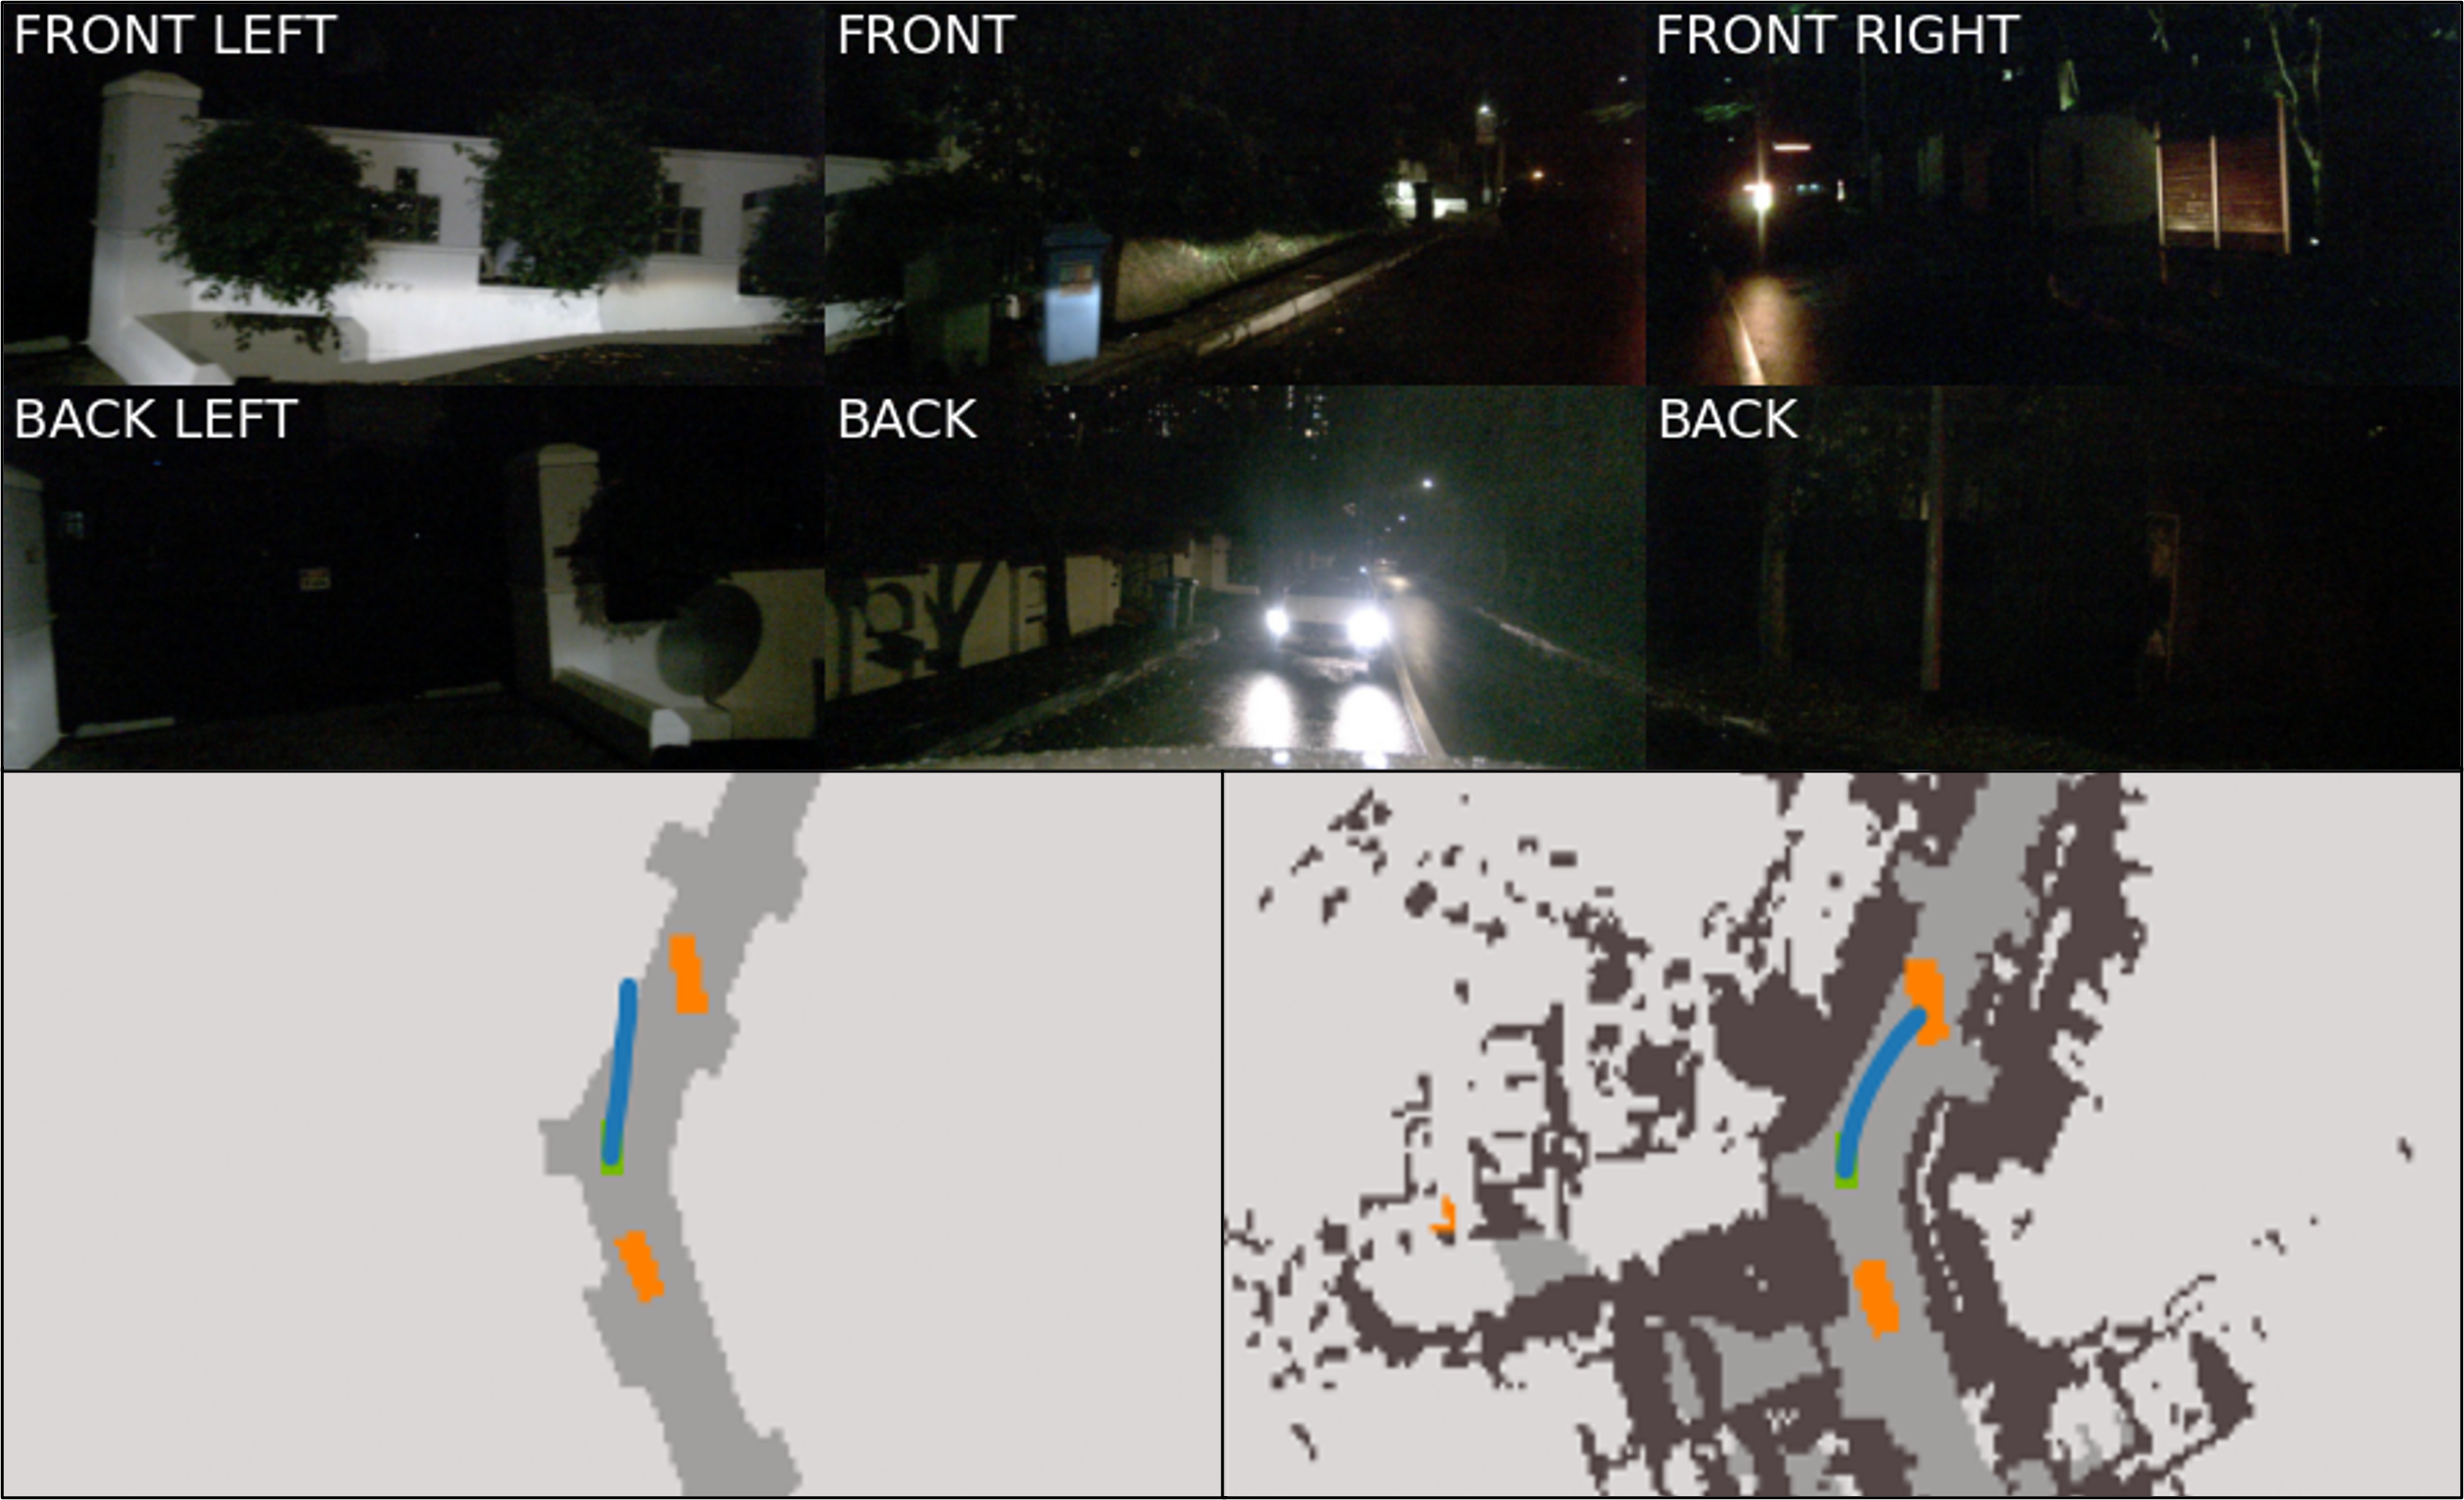
\includegraphics[width=0.8\linewidth]{ch-occnet/images/fig_planning_used.png}
  \caption[Visualisation of planning with boxes and occupancy]{\textbf{Visualisation of planning.} The blue line is the planned trajectory. The lower panels show the rasterised bounding boxes (left) and the rasterised occupancy (right) used as planning input.}
  \label{occnet:fig:planning}
\end{figure}

\paragraph{Occupancy for planning.} With the predictions of the upstream tasks, \ie boxes or occupancy, the final trajectory is obtained through the cost filter and the GRU refinement module of ST-P3~\cite{st-p32022} from BEV segmentation inputs, which we obtain by rasterising the outputs of OccNet in BEV space. We compare the rasterised boxes and the rasterised occupancy, both predicted by OccNet, and also the direct segmentation of ST-P3. For a fair comparison, we follow the setup of ST-P3 and keep only the vehicle and pedestrian classes. Rasterised ground-truth inputs are reported for reference. As Table~\ref{occnet:tab:planning} shows, filtering trajectories with ground-truth occupancy performs best. Among predicted inputs, occupancy gives the lowest collision rate at every horizon (0.21\%, 0.55\% and 1.35\% at 1\,s, 2\,s and 3\,s). Relative to boxes predicted by the same network, the collision rate drops by 15\%--22\% across the three horizons. Relative to the segmentation of ST-P3 it drops by 58\% at 1\,s, although the gap narrows at 3\,s (1.35\% \vs 1.49\%). Using all 16 occupancy classes further improves the L2 distance, to the lowest values among predicted inputs (1.29\,m, 2.13\,m and 2.99\,m). As Fig.~\ref{occnet:fig:planning} illustrates, planning with full-class occupancy makes decisions within the feasible area and avoids collisions with background objects.

\subsection{Analysis}\label{occnet:sec:analysis}

\begin{table}[t]
  \centering
  \caption[Efficiency and performance of the decoder designs]{\textbf{Efficiency and performance of the three decoder designs} on semantic scene completion (ResNet50). Measured on a V100 GPU.}
  \label{occnet:tab:efficiency}
  \begin{tabular}{lccccc}
    \toprule
    Method & mIoU$\uparrow$ & $\text{IoU}_{\text{geo}}$$\uparrow$ & Params$\downarrow$ & Memory$\downarrow$ & FPS$\uparrow$ \\
    \midrule
    BEVNet   & 17.37 & 36.11 & 39M & 8G  & 4.5 \\
    VoxelNet & 19.06 & 37.59 & 72M & 23G & 1.9 \\
    \rowcolor{perceive!10} OccNet & \textbf{19.48} & \textbf{37.69} & 40M & 18G & 2.6 \\
    \bottomrule
  \end{tabular}
\end{table}

\paragraph{Model efficiency.} Table~\ref{occnet:tab:efficiency} compares OccNet with the two extreme designs, BEVNet and VoxelNet, on semantic scene completion. OccNet obtains the best mIoU and $\text{IoU}_{\text{geo}}$ (19.48 and 37.69) with 40M parameters, nearly as few as BEVNet (39M) and far fewer than VoxelNet (72M). It also uses less memory than VoxelNet (18G \vs 23G) and runs faster (2.6 \vs 1.9 FPS on a V100 GPU); BEVNet is the cheapest design but the least accurate. The per-class comparison in Table~\ref{occnet:tab:occ_ablation} (Appendix~\ref{occnet:app:experiments}) shows the same ordering with ResNet101, with 24.62, 26.06 and 26.98 mIoU for BEVNet, VoxelNet and OccNet.

\begin{table}[t]
  \centering
  \caption[Detection versus occupancy on irregular objects]{\textbf{Detection versus occupancy on irregular objects.} $\text{mIoU}_{\text{ir}}$ is the mean IoU over truck, trailer and construction vehicle, with detected boxes converted to voxels.}
  \label{occnet:tab:irregular}
  \begin{tabular}{lccccc}
    \toprule
    Task & $\Delta s$ & $\text{mIoU}_{\text{ir}}$ & Truck & Trailer & Cons.\ veh. \\
    \midrule
    Det & 0.5\,m & 15.92 & 23.19 & 9.57 & 15.00 \\
    \rowcolor{perceive!10} Occ & 0.5\,m & \textbf{18.13} (\textcolor{red}{+2.21}) & \textbf{25.59} & \textbf{12.29} & \textbf{16.51} \\
    \midrule
    Det & 0.25\,m & 9.90 & 14.84 & 5.10 & 9.75 \\
    \rowcolor{perceive!10} Occ & 0.25\,m & \textbf{13.41} (\textcolor{red}{+3.51}) & \textbf{18.85} & \textbf{7.14} & \textbf{14.25} \\
    \bottomrule
  \end{tabular}
\end{table}

\begin{figure}[t]
  \centering
  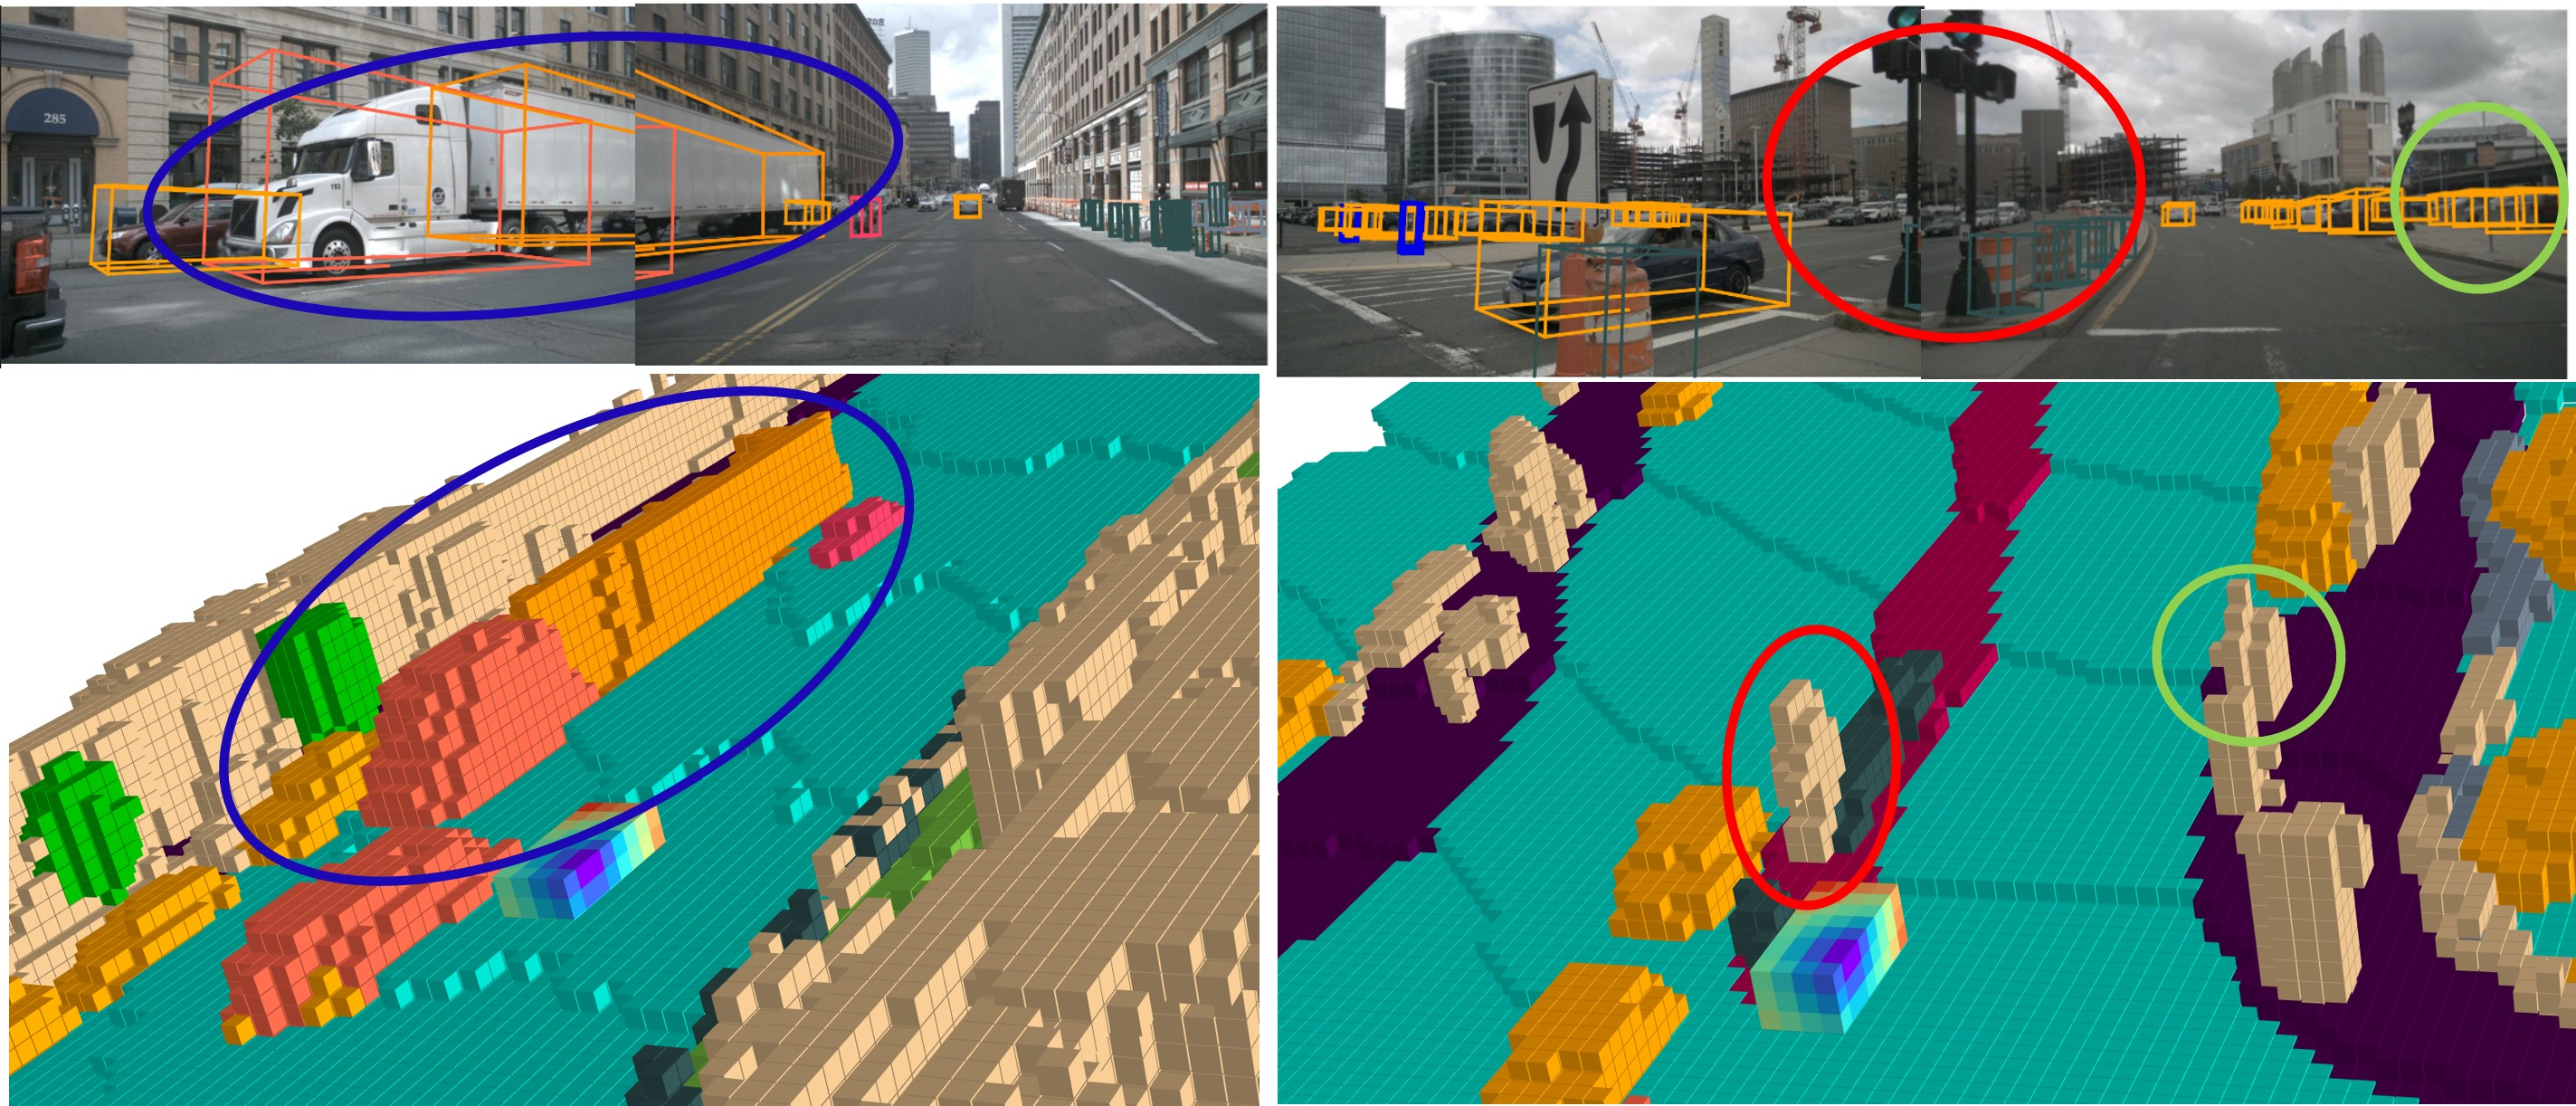
\includegraphics[width=\linewidth]{ch-occnet/images/fig_irregular_object_used.jpg}
  \caption[3D box and occupancy predictions for irregular objects]{\textbf{Visualisation of 3D box (top) and occupancy (bottom) predictions.} The ellipses highlight an irregular vehicle and background structures such as traffic signs, which are difficult to represent accurately with 3D boxes.}
  \label{occnet:fig:irregular}
\end{figure}

\paragraph{Irregular objects.} Representing irregular objects such as construction vehicles, or background stuff such as traffic signs, with 3D boxes is difficult and inaccurate, as Fig.~\ref{occnet:fig:irregular} shows. To compare detection and occupancy on irregular objects, we transform 3D boxes into voxels and evaluate both tasks on truck, trailer and construction vehicle (Table~\ref{occnet:tab:irregular}). Occupancy describes these objects better, with an $\text{mIoU}_{\text{ir}}$ of 18.13 against 15.92 for boxes at $\Delta s=0.5$\,m. To study the effect of voxel size, we also generate the dataset at $\Delta s=0.25$\,m. As $\Delta s$ decreases from 0.5\,m to 0.25\,m, the gap between boxes and occupancy grows from 2.21 to 3.51 points, because the finer granularity depicts irregular objects better.

\paragraph{Dense versus sparse occupancy.} Compared with sparse occupancy, dense occupancy depicts the complete geometry of background and foreground objects in detail (Fig.~\ref{occnet:fig:compare_gt}). Intuitively, dense occupancy is therefore better for 3D perception and motion planning, because it provides more abundant information. Fig.~\ref{occnet:fig:pretrain_for_detection} confirms that pre-training on dense occupancy generally benefits downstream 3D detection more than pre-training on sparse occupancy, most visibly when fine-tuning on 1/128 of the training set.

%-----------------------------------------------------------------------
\section{Discussion and Limitations}\label{occnet:sec:discussion}

\paragraph{What occupancy provides.} The experiments bear on the three requirements that RQ1 places on a scene representation. The first is validity beyond a closed vocabulary of boxes. Because occupancy does not presuppose object shape, it describes irregular vehicles better than boxes (Table~\ref{occnet:tab:irregular}), and it covers the background structures that boxes ignore. The planner of Section~\ref{occnet:sec:exploitation_of_occupancy} consumes binarised occupancy, so a cell contributes to the safety cost whenever it is predicted as occupied, whatever its semantic class; with all 16 classes, planning also avoids collisions with background objects (Fig.~\ref{occnet:fig:planning}). The semantics of occupancy, however, remain a closed set of 16 classes, so its openness lies in geometry rather than in recognition. The second requirement is learnability from cameras: OccNet predicts occupancy from images alone and approaches a LiDAR-based segmentation model (Table~\ref{occnet:tab:lidarseg}). The third is usefulness for planning: the better scene representation translates into fewer collisions (Table~\ref{occnet:tab:planning}).

\paragraph{Limitations.} Several limitations qualify these conclusions.
\begin{itemize}
  \item \emph{Dependence on an annotated dataset.} The annotations are still based on a well-established dataset: they rely on the LiDAR points and 3D boxes of nuScenes, including boxes interpolated for intermediate frames. Utilising self-supervised learning to further reduce the cost of human annotation is a valuable direction.
  \item \emph{Resolution.} A voxel size of 0.5\,m is too coarse for box metrics that depend on precise centres and IoU (Table~\ref{occnet:tab:joint_train}), whereas finer voxels describe irregular objects better (Table~\ref{occnet:tab:irregular}) and improve LiDAR segmentation (Table~\ref{occnet:tab:lidarseg_resolution}). The resolution of the representation therefore matters, and 0.5\,m is not fine enough for every use.
  \item \emph{Not every use of occupancy helps.} Features pre-trained on occupancy do not improve the planner over detection pre-training (Table~\ref{occnet:tab:planning_pretrain}); planning benefits when it consumes the predicted occupancy directly. Under an occupancy-based collision metric, occupancy input remains better in most intervals, but by small margins (Table~\ref{occnet:tab:occupancy_metrics}), and a cost function designed specifically for occupancy input may improve planning further. TPVFormer remains better on car, truck and trailer, and a camera-only model is still well below a strong LiDAR segmentation model (60.46 \vs 76.10 mIoU for Cylinder3D).
  \item \emph{Scope of the evaluation.} All experiments use nuScenes, planning is evaluated with the L2 and collision metrics of ST-P3 on logged data rather than in closed loop, and robustness under distribution shift, such as a change of city, weather or sensor set-up, is not evaluated.
\end{itemize}

\paragraph{Towards a foundation model.} We concluded the original study with the hope that the occupancy framework can become the foundation model of autonomous driving. A foundation model needs data at a scale and diversity far beyond the 850 scenes of nuScenes, which motivates the benchmark described next.

%-----------------------------------------------------------------------
\section{Scaling Up: The OpenScene Benchmark}\label{occnet:sec:openscene}

OpenOcc showed that occupancy can be learned from cameras and exploited across the driving stack, but it inherits the scale of nuScenes: like the other occupancy datasets built on nuScenes, it covers about 5.5 hours of driving (Table~\ref{occnet:tab:openscene}). For the foundation-model direction raised above, a large-scale dataset and benchmark is a must-have, and diversity matters as much as size; as the release put it, ``driving behavior on a sunny day does not apply to that in dancing snowflakes''. OpenScene~\cite{sima2023openscene} scales occupancy supervision to more than 120 hours of driving collected in four cities. It follows the benchmark-driven research cycle of Chapter~\ref{ch:methodology}: rather than collecting new data, it curates an existing corpus, adds a new supervision signal, and bundles it with metrics, a baseline, a development kit and challenges. OpenScene was released as a dataset with documentation rather than as a paper; the facts in this section are taken from its official documentation, which has evolved since the first release.

\paragraph{A compact redistribution of nuPlan.} OpenScene is built on nuPlan~\cite{caesar2021nuplan}, whose raw sensor data exceed 20\,TB, a size that is hard to handle for many academic groups. OpenScene is a compact redistribution that retains only the relevant annotations and sensor data at 2\,Hz, which reduces the dataset size by more than a factor of ten; the sensor data of the trainval and test splits amount to approximately 2\,TB. Its folder layout is aligned with nuPlan, so that users who already hold nuPlan sensor data can link it instead of downloading it again. The release covers 1,521 logs and more than 120 hours of driving in Las Vegas (64\%), Singapore (15\%), Pittsburgh (12\%) and Boston (9\%), split into 1,310 trainval, 147 test and 64 mini logs. It inherits the nuPlan scenario categories, which cover dynamics (5 types, \eg high lateral acceleration), interactions (18 types, \eg waiting for pedestrians to cross), zones (8 types, \eg pickup--drop-off areas), manoeuvres (22 types, \eg unprotected cross turns) and behaviours (22 types, \eg stopping at a traffic light with a lead vehicle ahead). Each frame provides images from eight cameras and a merged LiDAR point cloud.

\paragraph{Labels.} On top of nuPlan, OpenScene provides 3D bounding boxes, occupancy and flow annotations in 3D space. The occupancy labels use 0.5\,m voxels, the voxel size of OpenOcc, within $[-50\,\text{m},50\,\text{m}]\times[-50\,\text{m},50\,\text{m}]\times[-4\,\text{m},4\,\text{m}]$, and each label accumulates LiDAR frames over a window of 20 seconds. The flow annotation gives the motion direction and velocity of each occupancy grid cell. As with the flow of OpenOcc, the aim is to serve decision-making: in the words of the release, the motion information of occupancy flow ``can help bridge the gap between decision-making and scene representation''. The per-frame metadata include the ego pose and dynamic state, CAN bus data, the traffic-light status, a driving command (left, forward, right or unknown), camera intrinsics and extrinsics, and box annotations with velocities and with instance and track tokens. Tracks and ego states are provided at 2\,Hz, and scenes last 20\,s on average. The classes listed in the documentation are vehicle, bicycle, pedestrian, traffic cone, barrier, construction zone sign and generic object, plus background.

\begin{table}[t]
  \centering
  \caption[Scale of 3D occupancy datasets]{\textbf{Scale of 3D occupancy datasets}, following the comparison in the OpenScene documentation~\cite{sima2023openscene} (a subset of its rows is shown). Hours refer to the sensor data of the source database. $^{\dagger}$The documentation lists this dataset (as OccNet) without flow; OpenOcc annotates flow for foreground voxels (Section~\ref{occnet:sec:benchmark_overview}).}
  \label{occnet:tab:openscene}
  \begin{tabular}{llcc}
    \toprule
    Dataset & Source database & Sensor data (h) & Flow \\
    \midrule
    MonoScene~\cite{cao2022monoscene}                & NYUv2 / SemanticKITTI & 5 / 6     & \ding{55} \\
    Occ3D~\cite{tian2023occ3d}                       & nuScenes / Waymo      & 5.5 / 5.7 & \ding{55} \\
    Occupancy-for-nuScenes~\cite{Fang2023}           & nuScenes              & 5.5       & \ding{55} \\
    SurroundOcc~\cite{wei2023surroundocc}            & nuScenes              & 5.5       & \ding{55} \\
    OpenOccupancy~\cite{wang2023openoccupancy}       & nuScenes              & 5.5       & \ding{55} \\
    OpenOcc (Section~\ref{occnet:sec:benchmark})     & nuScenes              & 5.5       & \checkmark$^{\dagger}$ \\
    \midrule
    \rowcolor{perceive!10} OpenScene                 & nuPlan                & 120       & \checkmark \\
    \bottomrule
  \end{tabular}
\end{table}

\paragraph{Tasks and baseline.} The 2023 edition of OpenScene defined two tasks. The first is large-scale occupancy prediction, evaluated with the mIoU of Eq.~\eqref{occnet:eq:miou}. The second is an all-in-one foundation-model track scored by the OpenScene Metric, which averages nine downstream scores: 3D detection, semantic segmentation, scene completion, map construction, depth estimation, 3D lane detection, tracking, visual odometry and flow, measured with protocols from nuScenes, KITTI and Waymo. The occupancy baseline released with the benchmark is based on OccNet, with a ResNet-50 backbone.

\begin{figure}[t]
  \centering
  \begin{tikzpicture}[node distance=5mm and 9mm]
    \node[pillar=bench, text width=2.6cm] (nuplan) {\textbf{nuPlan}\\[1pt]1,521 logs, 120+\,h\\four cities\\raw sensor data\\$>$20\,TB};
    \node[pillar=perceive, text width=3.2cm, right=of nuplan] (os) {\textbf{OpenScene}\\[1pt]2\,Hz, $>$10$\times$ smaller\\8 cameras + merged LiDAR\\3D boxes, occupancy\\(0.5\,m) and flow};
    \node[pillar=act, text width=4.4cm, right=of os] (e2e) {\textbf{End-to-End Driving at Scale}\\[1pt]NAVSIM, PDM Score\\CVPR 2024; NAVSIM-v2, CVPR 2025};
    \node[pillar=perceive, text width=4.4cm, above=of e2e] (occ) {\textbf{Occupancy prediction}\\[1pt]mIoU, OccNet-based baseline};
    \node[pillar=arch, text width=4.4cm, below=of e2e] (wm) {\textbf{Predictive World Model}\\[1pt]ViDAR, Chamfer distance\\CVPR 2024};
    \draw[flow] (nuplan) -- node[above, note] {redistribute} (os);
    \draw[flow] (os.east) -- (occ.west);
    \draw[flow] (os.east) -- (e2e.west);
    \draw[flow] (os.east) -- (wm.west);
  \end{tikzpicture}
  \caption[OpenScene and its downstream use]{\textbf{OpenScene and its downstream use.} OpenScene redistributes nuPlan at 2\,Hz with occupancy and flow labels. It provides the data for large-scale occupancy prediction and for the end-to-end driving and world-model tracks of the CVPR 2024 and 2025 Autonomous Grand Challenges.}
  \label{occnet:fig:openscene_usage}
\end{figure}

\paragraph{Downstream use.} OpenScene became the data backbone of later benchmarks for end-to-end driving and world models (Fig.~\ref{occnet:fig:openscene_usage}). At the CVPR 2024 Autonomous Grand Challenge it supplied the data for two tracks. The \emph{End-to-End Driving at Scale} track was run with the NAVSIM development kit~\cite{dauner2024navsim}: a model receives camera images, LiDAR, ego states and navigation commands, and outputs a 4\,s trajectory, which is scored by the PDM Score after a 4\,s non-reactive simulation in which background actors replay the logs. The \emph{Predictive World Model} track, based on ViDAR~\cite{yang2024vidar}, asks a model to forecast point clouds for the next 3\,s from about 3\,s of past images and ego poses, and scores the forecasts by Chamfer distance. The private test sets of both tracks were provided exclusively by Motional. Version 1.1 of the dataset, released in March 2024, reorganised the metadata by nuPlan log and added raw LiDAR data; it also hosts the private test splits, including a hard split for the NAVSIM-v2 End-to-End Driving track of the CVPR 2025 Autonomous Grand Challenge. NAVSIM, on which Chapter~\ref{ch:centaur} evaluates test-time training for end-to-end driving, itself builds on OpenScene and nuPlan. The data infrastructure built for occupancy in this chapter thus also underpins the end-to-end driving evaluation later in this thesis.

\paragraph{Limitations.} The documentation of OpenScene leaves several gaps. The number of semantic occupancy categories was still marked as to be determined in its comparison table, and the annotation procedure is documented only partially beyond the 20-second LiDAR accumulation. Occupancy labels are distributed with version 1.0, and a few frames of version 1.1 lack them. No peer-reviewed study of the label quality has been published. The data are skewed towards Las Vegas (64\%), and they are licensed for non-commercial use only (CC BY-NC-SA together with the nuPlan licence).

%-----------------------------------------------------------------------
\section{Chapter Summary}\label{occnet:sec:summary}

This chapter answered RQ1 by proposing 3D occupancy as a general scene descriptor for autonomous driving. Instead of enclosing a closed set of object categories in boxes and flattening the background into a BEV map, occupancy quantises the space around the vehicle into voxels with semantic labels and flow, so that objects of any shape and structures above the ground are described in one grid. We presented OccNet, which reconstructs occupancy from surround-view cameras by lifting BEV features to voxels step by step with a cascade voxel decoder, voxel-based temporal self-attention and 3D deformable attention; OpenOcc, a dense occupancy benchmark on nuScenes with 34,149 frames, over 1.4 billion voxels in 16 classes, and flow for foreground objects; and OpenScene, which scales occupancy and flow supervision to more than 120 hours of nuPlan driving and later provided the data for NAVSIM and for the CVPR 2024 and 2025 Autonomous Grand Challenges.

The experiments support the three requirements of RQ1. Occupancy is learnable from cameras: OccNet reaches 26.98 mIoU and 41.08 $\text{IoU}_{\text{geo}}$ on OpenOcc, against 23.67 and 37.47 for TPVFormer, and from cameras alone it reaches 60.46 mIoU in LiDAR segmentation, comparable with the LiDAR-based RangeNet++ (65.50). Occupancy describes irregular objects better than boxes, and its advantage grows from 2.21 to 3.51 $\text{mIoU}_{\text{ir}}$ as the voxel size shrinks from 0.5\,m to 0.25\,m. Occupancy is useful for planning: planning on predicted occupancy gives collision rates of 0.21\%, 0.55\% and 1.35\% at 1, 2 and 3\,s, against 0.27\%, 0.68\% and 1.59\% with predicted boxes. The cascade decoder achieves this with 40M parameters, close to the 39M of a BEV-only design. The limitations are equally clear. The labels still derive from an annotated dataset and its LiDAR; features pre-trained on occupancy do not help the planner, which benefits only from consuming the predicted occupancy directly; a camera-only model remains behind a strong LiDAR segmenter (76.10 mIoU for Cylinder3D); and all experiments use a single dataset and open-loop planning metrics, without evaluating distribution shift.

Occupancy tells the agent \emph{what is where}. It does not tell the agent \emph{why} a situation matters or \emph{what to do} about it. The same occupied voxels describe a pedestrian at the kerb whether or not that pedestrian intends to cross, and a stopped vehicle ahead whether it is parked or waiting at a red light, yet each case calls for a different decision. Answering such questions requires general knowledge about how traffic works, and reasoning that connects perception to the prediction of other agents and to the planning of the ego vehicle. This motivates Chapter~\ref{ch:drivelm}, which grounds the general knowledge of vision-language models in driving through structured, verifiable reasoning that proceeds from perception through prediction to planning.
